\chapter{Cross-Blockchain Protocol for Public Registries}

\begin{center}
{\large\uppercase{$\text{Oleksii Konashevych}^{[0000-0003-0068-5962]}$}} 

Erasmus Mundus Joint International Doctoral Fellow in Law,\\ Science and Technology. 

\vskip -6pt

\end{center}

\vskip 2cm




\vfill




\newpage

\begin{multicols}{2}

\section*{Abstract} 

This paper presents a concept of the protocol for public registries based on blockchain. The proposed mechanism allows creating a standard database over a bundle of distributed ledgers. It ensures a blockchain agnostic approach and utilizes the benefits of various blockchain technologies in one ecosystem. In this scheme, blockchains play the role of journal storages (immutable log), while the overlaid database is the indexed storage. The distinctive feature of such a system is that in blockchain, users can perform peer-to-peer transactions directly in the ledger using blockchain native mechanism of user access management with public-key cryptography (blockchain does not require to administrate its database). The protocol can be used to develop public property registries, i.e. land titles, cars, boats, corporate rights, etc. Users can create and manage their rights using the full power of blockchain technologies and smart contracts. The component of governance in this protocol is introduced as Smart Laws and Digital Authorities, the algorithms to manage the overlaid system and address legal issues with property rights and law enforcement.

\textbf{Keywords:} blockchain, electronic government, public registry, land registry, smart law, digital authority

\section{Introduction}\label{sec-01}
 
Governments play a crucial role in keeping public registries to prevent legal disputes about “who owns what.” Thus, the government acts as a trusted third party in private relations. However, if the government as a mediator loses the ability to be a source of law and order, it becomes a cause of conflicts.

Therefore, centralization, for instance, in state-owned land registry is a solution, but a source of risks. Risks are addressed by a system of hierarchically organized public administration, separation of powers, multiple checks and balances. It all becomes a burden for citizens that pay taxes and deal with red tape.

For a quiet time, it prevails Weber’s doctrine of the inevitability of bureaucracy \cite{art1-key01}. He believed that at this point of development, society should accept bureaucracy as inevitability and necessity.

The idea of the blockchain\footnote{The word “blockchain” is used here in the original meaning, i.e., a decentralized, uncensored public system. Hence, “permissioned” and “private” DLTs due to their centralized nature are not blockchains. Therefore, governments that use centralized technologies cannot claim the application of blockchain.} use for state-level governance and public registries is an open space for discussion in academia and blockchain industry, because it may reduce centralization.

A conceptualization in this field so far was limited to general ideas of “disrupting governance” (regulations, bureaucracy, middlemen, among others.) superficial in their essence, and unable answer how to design the system where law and technology will not collide exposing existing problems: enforceability in an immutable ledger of the blockchain technology, scalability, sustainable governance and many more discussed below.

Cross-Blockchain Protocol (CBP) is the technology of an overlaid database across a bundle of ledgers that enables smart laws and enforceability. The protocol is fundamental for the use of blockchains for property registries (for example, land cadastre) and other public databases run by governments. It may also have applications in the private and commercial sphere.

Alternatively, to an open and decentralized blockchain technology, tech consortia propose governments so-called “permissioned” (also known as private, federated, enterprise, etc.) Distributed Ledger Technologies (DLT), which are centralized, have similar vulnerabilities and limitations which other centralized technologies have. The advantages of such systems DLTs are questionable. There is no convincing evidence why this kind of technology is better than those centralized systems that governments have used for decades. It ensures immutability for records at the discretion of the authorities, i.e., retroactivity, censorship, corruption, and even full-stop of services are possible depending on a specific design of a system.

Moreover, DLTs have some unique features and some trade-offs, which may address one problem but will not be suitable for another. There is no reason to believe that any particular DLT is better than others and there will be one ultimate ledger. Hence, why would the government choose one DLT in favor to others?

But the major question in any technological shift is the cost of a mistake. Will governments have an opportunity to shift back or choose alternative technology with reasonable costs if anything goes wrong?

While one government agency runs one permissioned DLT solely, there is obviously no decentralization. If instead, a private network is in use, why would the government allow one private infrastructure provider (or a consortium) to monopolize the domain of public services?

Other questions may also arise. For example, if this is constitutional at all to share government sovereignty with a closed group of providers (nodes) that run a private network to provide public services? 

And finally, if a bunch of decent competitive and secure networks can provide reasonable infrastructure for public services, why choose one but not all?

Public blockchains, even though they are decentralized, it is not static.  Decentralization is ensured by constant fair competition. Bitcoin, Ethereum and some other public networks show that they remain sustainable. If some troubles happen on their ways, they still can tackle them without any central authority. Decentralization is the guarantee of the records to be safe and immutable. Centralized databases cannot provide such a level of immutability.

Therefore, this research is based on a hypothesis that public blockchains can be used as storage for records of land rights and other property rights (which normally are stored in government databases) and various government services, which also involves the need to store data in public databases.

Though immutability is not the only advantage. The traditional database cannot provide direct access for end-users; transactions are performed through registrars. Blockchains have a native mechanism to manage ownership with public key cryptography and the user can perform peer-to-peer transactions (title deeds). Thus, the user needs neither registrars nor registry keepers.

Once a token which represents the land title of the owner is created on the blockchain, there is no need to keep track of its transactions elsewhere. There is no need in any land registry because blockchain is the registry itself.

Nevertheless, people still need legal procedures, which now exists in paper form and applied by those registrars and other public bodies. Hence, the combination of blockchain and automation of procedures may significantly improve governance.

Such ideas remain for a while hypothetical, but this research is the first attempt to introduce a systematic approach of a system architecture for public services.

The proposed protocol aims to ensure that within the created bundle of existing blockchains, not the government, but citizens decide themselves where to keep their records of ownership and manage property rights. The bundle may unite not only public ledgers, but also permissioned, private, etc., and also interact with closed, centralized databases, which makes possible a shift from mono-database run by the government agency to multiple ledgers and cross-chain transfers.

This ensures fair competition among technologies, because users not only may choose any ledger within the bundle but transfer their assets from one chain to another if any technology does not suit their interests. On the other side, there is no need for the government to decide for citizens which technology to use, which corresponds with the principle of technological neutrality.

The protocol is a standard that transforms the “wild west” of incompatible and non-interactive networks into unified ecosystem. Notably, it does not require upgrades or permissions of these networks for the protocol to be applied.

Straightforward use of blockchain for running public registries is impossible. There are legal issues with enforceability and immutability, hardforks, digital identity, privacy, scalability and price volatility. The protocol is designed to address them.

It introduces the concept of “smart laws.” This is a framework for smart contracts and enforcement. Smart laws consist of algorithms that enable digital authorities to address legal issues: disputes, inheritance, loss of private keys, etc.

\section{Theoretical Framework,\\ Methodology and Literature\\ Review}\label{sec-02}
\subsection{Methodology and Theoretical\\ Framework}\label{subsec-02.1}

This paper is framed with design science research (DSR) provided by Hevner et al. \cite{art1-key02}. As per DSR, the research is meant to present an “artifact” which is defined as “constructs (vocabulary and symbols), models (abstractions and representations), methods (algorithms and practices), and instantiations (implemented and prototype systems).” This research deals mostly with \textit{models} and \textit{methods}.

In particular, the cross-blockchain database is a model, and cross-blockchain protocol is a set of methods of how this model can be designed. The research provides for a broad discussion and evaluation of the applicability of the proposed invention and constructs various models of its use in governance.

This research is complaint with 7-step research guidelines provided by Hevner et al., and corresponds with Design Science Research Publication Schema \cite{art1-key03} by Gregor and Hevner. The following table outlines steps of the performed SDR:

The following table outlines steps of the performed SDR: \textit{Method}. The primary method for this DSR is \textit{exaptation}, i.e., adoption of solutions from other fields. The research is looking into existing technologies which are applied here as elements of the protocol: Name-Value Storage, Berkley DB, RAID protocol, among others. The choice of Name-Value Storage as a reference technology for creating a database over blockchain is based on the analysis and comparison with two other similar technologies Bigchain and Amazon QLDB, presented in Section~\ref{subsubsec-4.1.a}.
\end{multicols}
\begin{center}
\begin{tabular}{|l|l|m{13cm}|}
\hline
\textbf{\#} & \textbf{Step} & \textbf{Comment}\\\hline
1 & Introduction & Section 1 - the purpose and scope of the artifact – present a public registry model for property rights based on a bundle of existing public blockchains with enforcement and interoperability. Section 3 presents issues of the blockchain use by governments, which forms a corpus of research questions, which are to be addressed by this DSR.\\\hline
2 & Literature review & Subsection 2b provides context to the relevant academic research in blockchain and governance to support the integral elements of the protocol and proposed methods.\\\hline
3 & Method & Subsection 2a (this subsection)\\\hline
4 & Artifact description & Section 3 - a design concept of a cross-blockchain protocol for the creation of end-to-end public databases across a bundle of blockchains.\\\hline
5 & Evaluation & Subsection 4.3 is a technical evaluation of the architecture, its limitations and strategies to manage risks and constraints.\\\hline
6 & Discussion & Section 5 is a general evaluation of the technology applicability with legal and political aspects.\\\hline
7 & Conclusion & Section 6 is a summary of the research outcomes and discussion of further directions of the research.\\
\hline
\end{tabular}
\end{center}
\begin{multicols}{2}
The evaluation does not use experimental and testing methods for a few reasons. Firstly, there are no quantitative objectives (for example, there are no purposes to improve latency performance, bandwidth or size transaction optimization, among others); hence, there is nothing to measure for evaluation.

Secondly, the creation of a key-value DB across a bundle of public repositories is feasible enough to argue its implementation possibility.

The theoretical value of this research is more important since it meant to present viable models and scenarios of the use of decentralized blockchains, instead of permissioned DLTs in the public sector. The absence of any solution in this space practically makes the application of the public blockchain impossible, for instance, for property registries, due to known legal issues. Therefore, the hypothetical concept is valuable as it opens a discussion in the field.

Lastly, the development of the running system may require substantial resources. Therefore, broader independent evaluation and contribution among researchers many create more knowledge to consider development prototypes in the future.

Therefore, this research was focused on designing the concept of the protocol and, more generally, the concept of public registries across multiple blockchains, while all elements of this architecture exist and tested in various other applications.

\subsection{Literature review}\label{subsec-02.2}

Recent academic literature creates a valuable context on the blockchain use, its benefits, applications, characteristics, classification and constraints.

The paper “Constraints and benefits of the blockchain use for real estate and property rights” \cite{art1-key04} became a basis for this research because it identified major constraints of the emerging technology for a public property registry, which laid down as the purpose to address in this research, i.e., to find the way to utilize benefits of blockchain for public property (real estate, land, etc.) registry and overcome major constraints (see Section 3).

A large portion of papers operate on a higher level when it comes to land registry, i.e., public services and e-government, seeking answers on how blockchain can improve this field. Among the first to discuss governance and blockchain was a journal paper “Beyond Bitcoin enabling smart government using blockchain technology” \cite{art1-key05} by Ølnes (2016). The author refers to the example of publishing hashes on Bitcoin - a small project at the University of Nicosia, where students were given electronic certificates after finishing a course, and a hash sum of the certificate was inserted in Bitcoin’s blockchain. Hashing on blockchain is much discussed in “Blockchain Anchoring of Public Registries: Options and Challenges” \cite{art1-key06}. The authors discussed  requirements for better system architecture for centralized public registry and DLT over it to hash DB entries.

In “Disrupting governance with blockchains and smart contracts,” \cite{art1-key07} Shermin (2017) discusses the major constraints of the use of blockchain. There is a gap between the initial conceptualizations of blockchains and their first instantiations. First use cases show that as circumstances change, protocols can become inappropriate for the new environment and require modification. Modification of blockchain code happens through majority consensus, but reaching consensus in a distributed multi‐stakeholder network with sometimes unaligned interests is complex, potentially introducing new agency issues.

In “Blockchain technology as a support infrastructure in e-Government,” \cite{art1-key08} Ølnes and Jansen (2017) continued the exploration of blockchain for governance. The authors are among the first to caution unreasonable optimism in the use of “permissioned” and “private” systems in public services: “Closed blockchains [...] must rely on traditional security mechanisms in order to prevent unwanted access and modification to the blockchain.” The paper mainly discusses open blockchains [networks], because as authors emphasize, “closed systems are never able to build an infrastructure.”

In “Blockchain in Government: Benefits and implications of distributed ledger technology for information sharing,” \cite{art1-key09} Ølnes, Ubacht and Janssen (2017) ask whether blockchain technology will lead to innovation and the transformation of governmental processes. To address this question, the authors presented a critical assessment of the “often exaggerated benefits of blockchain technology” found in the literature and discussed their implications for governmental organizations and processes. The paper summarizes directions for further research into the potential benefits of blockchain applications in e-government and the role of governance of blockchain architectures and applications to comply with societal needs and public values.

In “A framework of blockchain-based secure and privacy-preserving E-government system,” \cite{art1-key10} Elisa et al. (2018) argue that most of the existing e‑government systems, such as websites and electronic identity management systems (eIDs) are centralized at duplicated servers and databases. A centralized management and validation system may suffer from a single point of failure and make the system a target to cyberattacks such as malware, denial of service attacks (DoS), and distributed denial of service attacks (DDoS). The blockchain technology enables the implementation of highly secure and privacy-preserving decentralized systems where transactions are not under the control of third-party organizations. They propose a framework of a decentralized e-government peer-to-peer system using blockchain technology to ensure information security and privacy while simultaneously increasing the trust of the public sectors. In addition, a prototype of the proposed system is presented with the support of a theoretical and qualitative analysis of the security and privacy implications of such a system. It is important to note that the authors share the idea that a “permissioned” (centralized) system can be called “blockchain.” They attribute this system features of blockchain: “The permissioned blockchain system ensures that the stored records are trustworthy, auditable and transparent.” In the proposed architecture, it is clear that infrastructure is introduced and maintained by the government. The question of how the proposed centralized system is better than the existing one remains open.

Batubara, Ubacht and Janssen published their “Challenges of blockchain technology adoption for e-government: A systematic literature review” \cite{art1-key11} in 2018. The paper guides through a number of studies and pilots in the use of blockchain in governance available by 2018. Several countries such as the USA, the United Kingdom, the Netherlands, the United Arab Emirates, Estonia, Sweden and China announced blockchain initiatives to explore its uses in the public sector actively. Their findings have shown that academic research in this area had only just started and issues discussed in the selected literature were still significantly limited. Consequently, more intensive research in this area was still necessary to advance this field's maturity. As per the authors, the major challenges from the organizational perspective are the need for new governance models and the acceptability of this technology. The research into blockchain technology standards and a reference architecture for e-Government applications was proposed to resolve the technological challenges.

Further directions are found in Franciscon et al. (2019) “A systematic literature review of blockchain architectures applied to public services” \cite{art1-key12}. This work provides a systematic review of blockchain-based applications across multiple domains: supply chain, business, healthcare, IoT, privacy, and data management. Authors point to the shortcomings identified in the relevant literature, particularly limitations the blockchain technology presents and how these limitations spawn across different sectors and industries. Building on these findings, authors identify various research gaps and future exploratory directions that are anticipated to be of significant value both for academics and practitioners.

 Brinkmann and Heine (2019) in “Can blockchain leverage for new public governance? A conceptual analysis on process level” \cite{art1-key13} presented the preliminary results of ongoing research, which aimed to shed light on the more concrete benefits of Blockchain for the purpose of New Public Governance (NPG). The preliminary results show that Blockchain offers valuable support for governments seeking methods to coordinate co-producing networks effectively. It becomes evident that there is a need for off-chain processes. Therefore, it is argued in favor of intensifying research on off-chain governance processes better to understand the implications for and influences on on-chain governance.
 
More recently, the paper “Smart Contracts for Government Processes: Case Study and Prototype Implementation” \cite{art1-key14} by Krogsbøll et al. (2020) contains a description of the pilot with the Danish Municipality. The government partner concluded that the risk of losing access to the system (due to loss of private keys) outweighed any benefits. The researchers on the other side think that smart contract implementations of government processes need to be immutable and outside of the government’s control when running; however, they also need to be updatable when laws change and provide an “out” for the rare case when errors in the contract implementation result in unlawful behavior and consider these problems as the “foundational research challenge for blockchain to be applicable to governmental processes.”

To sum up, the recent research introduced a variety of opinions about the blockchain technology, its features, benefits, and limits. This creates grounds for further research and development, especially application in various spheres of economic activity far beyond cryptocurrency. Yet to be noticed; still, a lot of perspective ideas remain in theoretical phases, or early stages of piloting. Therefore, the future challenge is to observe, collect and analyze more empirical data to define better practices and pitfalls across multiple fields and disciplines.

\vspace{-.1cm}

\setcounter{secnumdepth}{5}
\renewcommand\thesubsubsection{\arabic{section}.\arabic{subsection}.\alph{subsubsection}}
\section{Public blockchains issues}\label{sec-03}

This section defines problems on the way of the blockchain use for public registries: risks of multiplication of assets due to hardforks, enforceability, anonymity, digital identity, privacy, data integrity, scalability and price volatility. In the end, it is summarized what is opposed to blockchains and why blockchain is still a good choice for infrastructure.

\vspace{-.2cm}

\subsection{Why blockchain is impossible to use in public service as it is}\label{subsec-03.1}

\vspace{-.2cm}

\subsubsection{Hardforks}\label{subsubsec-03.1.1}

\vspace{-.3cm}

The hardfork is the major concern for systems with open competition because there are no authorities that impose and enforce one exclusive status quo. 

The system can split into two or more branches or so-called “forks,” after which each branch becomes independent but has a spare history of transactions till the moment of fork.

In the result of the split, tokens are duplicated. For example, if the system is used to manage rights on movable or immovable property (often mentioned as “asset-backed tokens”), in the result of a hardfork, the user will still have one plot of land but two title records in parallel systems. In the result of the fork, they can be managed independently, thereby creating legal collisions. For example, in one system, the user sells the plot, but in the other, the user still owns it.

\vspace{-.7cm}

\subsubsection{Immutability}\label{subsubsec-03.1.2}

\vspace{-.4cm}

Being an advantage of blockchain technology, the immutability of the ledger can cause a lot of untoward use cases. For example, the loss of private keys will make cryptocurrency, a token, or a smart contract uncontrolled with negligible possibilities ever to restore it. Even if the blockchain can prevent many ownership disputes, the imperfect nature of people’s relationships will always cause issues with ownership and the need to settle when they arise. The blockchain itself, in its pure design, does not leave practical possibilities for enforcing any legitimate judicial decisions or any legal actions by authorities.

\vspace{-.7cm}

\subsubsection{Anonymity (pseudonymity)}\label{subsubsec-03.1.3}

\vspace{-.4cm}

The authorization and authentication for a transaction are provided only with the relevant private key within the asymmetric pair owned by the user. The public key of the pair is taken to generate the address. The concept of addresses is the cornerstone of the blockchain. In the result of a transaction, a coin is spent from one address and added to another address, but to enable such transfer, the owner of the coin must use the relevant private key. Thus, the address is the only public record in the ledger that identifies the user. 

However, some research showed that addresses could be deanonymized by different digital fingerprints found in the network (IPs, behavior patterns, among others.) \cite{art1-key15}, \cite{art1-key16}. The pure blockchain protocol is not suitable for keeping records on property and securities from the perspective of governments — blockchain anonymity veils money laundering, financing terrorism, and other unlawful activity.

Beyond that, at the practical level, the censorless nature of the blockchain creates confusion in identifying records. Anyone may perform any transaction and publish any data in the blockchain. If the government must authorize a land title deed, how do you define if any transaction on the blockchain belongs to the town clerk if they are all pseudonymous? Without overlaid solutions for digital identities and trust services, it is almost impossible to create any scalable model for governance.

\vspace{-.7cm}

\subsubsection{Data integrity, off-chain data and issues of\\ personal data}\label{subsubsec-03.1.4}

\vspace{-.4cm}

In blockchain, any published data is exposed, and removal is not an option. Alternatively, users can insert into the blockchain cryptographic hashes of the data. The blockchain that stores hash sums will provide for two things: the user can verify the authenticity of the data (whether it is still the same or not) and timestamping because blocks are chronologically stored.

However, hashing does not ensure the protection of the data itself. Once it is tampered with and/or deleted, the hash sum is useless for restoring. This leads to two possible solutions: data will be stored by the third party (for instance, a government agency) or users themselves.

Today all personal data and property records (title records) are stored in closed databases controlled by governments, and publishing hashes whether into the centralized DLT or open blockchain does not add much security. To verify this data, the user needs access to that closed database or just blindly trusts the entity which stores it.

Even if public blockchain is used to store hashes, there is still in this scheme a trusted party as the source of “truth,” and so concentrating many risks for leaks and corruption of data as a single point of failure.

\vspace{-.7cm}

\subsubsection{Scalability}\label{subsubsec-03.1.5}

\vspace{-.4cm}

One exclusively chosen blockchain for governance will necessarily create issues. Again because of the open and free nature, the blockchain protocol does not restrain publishing junk data in the ledger.

The potential bandwidth of Bitcoin per year, for example, is roughly 220 million transactions \cite{art1-key17}. For instance, 300 public registries in Ukraine generate as much as Bitcoin’s bandwidth \cite{art1-key18}, which leaves no space for other cryptocurrency transfers.

Overload with the transactions creates the problem of high transaction fees and price volatility. Although Bitcoin is not the best in terms of bandwidth, it is still the most attractive in terms of security \cite{art1-key19}. This is not a workable solution on a scale, even for one country with a 40-mln population, randomly chosen as an example.

For blockchain using other consensus protocols or other data structure, scalability is not the main issue. For example, Ethereum, IOTA, NXT, NEM, and many other systems ensure better bandwidth and performance.

The choice of one network in favor of others is a discussion about technological neutrality – a principle that is often discussed in the context of public policy. The reader may find discussions that compare one specific blockchain network with some specific centralized system, where usually blockchain performance is fewer. Having in mind the principle of technological neutrality, it is proposed to consider the problem of scalability from another perspective. One blockchain network does not necessarily provide enough scalability, while a bundle of blockchains may become much more effective.

\vspace{-.7cm}

\subsubsection{Price volatility}\label{subsubsec-03.1.6}

\vspace{-.4cm}

Due to speculations, the price can dramatically fluctuate; therefore, creating a bad user experience for those who need cryptocurrency to pay fees for publishing and managing data and running smart contracts. Together with the mentioned scalability issues, it makes it infeasible for the government to use or even to announce their intention to use any specific blockchain. It will inevitably incentivize agiotage on the market, exacerbating the problem of scalability even more.

\subsection{What is opposed to blockchains and why it is still a good idea to use them}\label{subsubsec-03.2}

Eventually, as might be thought, the permissioned DLT is much better than the blockchain, as it addresses all these issues due to its centralized nature, purposed to control and restrict unwanted practices and manually fix troubles.

There is no one specific consensus for permissioned systems. This is rather a title of various design concepts aimed to leave the leverage of control over the network in the hands of an authority, which can be by one actor or a closed group of actors.

Some protocols were not initially developed for permissioned design. For example, the Proof-of-Stake protocol (PoS) \cite{art1-key20} is designed as a cheaper alternative of Proof-of-Work. In PoS, network if a node (or a group of nodes who mutually agreed) has enough stake at their control, they may perform retroactive actions by rolling back blocks \cite{art1-key21} and can censor transactions.

Proof-of-Authority \cite{art1-key22}, and a family of Hyperledger consensuses \cite{art1-key23} protocols are dedicated to architecture with controlling features.

It is possible to design different schemas with privileged (“master”) nodes that are authorized for the creation of blocks, writing transactions, and some other specific rights providing those other participants of the network will not have them. Such systems can also be closed; therefore, users will need the authorization to read the information from blocks, whereas some protocol provides anonymous interaction (see, for example, DLT Quorum \cite{art1-key24}). Compared to existing centralized closed government systems, such DLTs may have some advantages; however, conceptually, they are the same. They are centralized and censorable and are not necessarily immutable for those who control it.

Another reason why the choice of one DLT leads to centralization is that the choice of one exclusive network prevents competition. By choosing a permissioned DLT, the government takes responsibility for developing and maintaining infrastructure.

On the contrary, open blockchain systems do not have central authorities that build the network. Any user is free to add their computational resources for public needs and therefore, compete for having rewards for finding blocks, and this reward is not distributed by someone centrally but automatically obtained as per the protocol. The infrastructure is self-organized incentivized by cryptocurrency with free competition for mining, i.e., creating and storing blocks.

The principle of decentralization is the basis of this research; therefore, we neither argue nor compare blockchain to centralized solutions. Centralized databases have already been in use for quite a long time by governments; therefore, we already know their advantages and disadvantages. Therefore, permissioned systems cannot be considered a significant evolutionary step in government systems.

Blockchain is a new word in governance, but this technology has some principal features that can restrain its implementation at the state level, and the following research conceptualizes ideas to address them.

Among various properties of the blockchain technology, we distinguish the following highly considerable for a new generation of public property registries:

\vspace{-.4cm}

\begin{itemize}
\item[-] Blockchain provides an append-only type of database, which is called an immutable ledger. It prevents data corruption and unauthorized changes.
\item[-] Blockchain has a native mechanism for managing ownership through public-key cryptography; thus, it is not only an immutable storage, but also it is a system for peer-to-peer transactions. On the contrary to traditional, for example, real estate registry, it does not require a trusted third party to record a deed in the database.
\item[-] Blockchain is self-organized and does not require central authorities to govern and maintain the infrastructure.
\end{itemize}

The proposal in this research concept utilizes the immutability of the blockchain with the help of “smart laws.” It reduces centralization when possible and makes it accountable when centralization is inevitable.

\section{Building a database across\\ blockchains}\label{sec-4}

The first subsection introduces an idealistic design model of a database across a bundle of blockchains (Subsection~\ref{subsec-4.1}). Subsections~\ref{subsec-4.2} and \ref{subsec-4.3} analyze constraints of the model and evaluate possible design solutions to get the system working.

\subsection{General idea and basic elements}\label{subsec-4.1}

\vspace{.1cm}

\subsubsection{General idea}\label{subsubsec-4.1.a}

A cross-blockchain database is a logic superstructure over a bundle of blockchains, see Figure~\ref{chap1-fig01}. To create a mutual interaction, users should agree which blockchains they include in the bundle and according to which rules and filters - the cross-blockchain protocol - they create the database.

The designed system collects users’ records from the blockchains of the bundle into a consistent end-to-end public database. The “record” is an entry the user inserts into any blockchain in the bundle, it can be a token (or a “colored coin”) or a key-value record.

An entry must be compliant with the format so the algorithm will automatically select and send in into the cross-blockchain database from heterogeneous data flow in blockchains (take into account that blockchain is uncensored; therefore, a lot of chunk data is also published there). This is the role of the protocol. It scans upcoming blocks in every ledger of the bundle and searches for records of a specific standard. 

It verifies each record as per the rules provided by the protocol and filters out if a record is non-complaint. Eventually, the system inserts the complaint record into the database, which is a local file on the user’s computer.

When a user applies the same protocol on any computer, he or she will receive the same copy of the database that every other user has on their local computers. Thus, there is no mathematical consensus for the database itself. The database relies on existing consensus protocols of those ledgers, which are included in the bundle. 

The consensus of the overlaid structure is a sort of a social contract because users must agree on the initial architecture of any particular database: which ledgers to scan and from which blocks, the format of the entry, and filtering rules, how to add new ledgers and drop a ledger from the bundle, how to transfer entries from ledger to ledger, how to upgrade and create patches in the protocol by collective decisions or by a central authority, etc. Thus, by applying the protocol and scanning blocks, users independently build a copy of the database.

\begin{figure}[H]
\centering
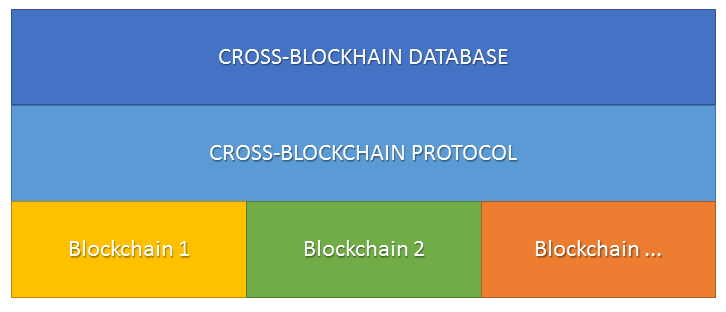
\includegraphics[scale=1.5]{src/Figures/chap1/chap1-fig01.jpg}
\caption{Basic scheme of a bundle of blockchains with overlaid database}\label{chap1-fig01}
\end{figure}

\begin{quote}
The bundle can contain any number of ledgers but at any point in time, the list must be definite. The protocol provides for format rules and filters for entries and rules for scanning, adding new and deleting included ledgers intro the bundle. The system scans block across ledger of the bundle and hooks records that are compliant with the rules and adds them to the database.
\end{quote}

\vspace{.1cm}

The blockchain provides for a native mechanism of ownership through public-key cryptography: the user publishes a record and the protocol considers the address from which he or she created this transaction as the owner of the record. Thus, to perform any update, the user must create a new record using the same private key because the private key is the authorizing mechanism for the address.

\vspace{.1cm}

This mechanism was developed by a number of blockchain projects. To better explain this protocol, let us refer to Emercoin’s Name-Value Storage (NVS) technology, which is working since 2014 as one of the successful designs for storing arbitrary users’ data in the structured form in the database. Emercoin’s itself became a successor of a Namecoin’s non-ICANN TLD service (Top-Level Domain “.bit”).

\vspace{.5cm}

It should be noted that other types of databases and technologies may be applied, and therefore, it will require a compatible format of a DB entry.

Emercoin’s NVS protocol details are specified in Annex. We can extract a set of useful elements of both Emercoin’s and Namecoin’s NVSs. The following subsection presents which elements should be taken as a basis for a cross-blockchain protocol.

To address the legitimate question of why other types of blockchain-enabled databases, for instance, Bigchain and Amazon QLBD, were not chosen as a reference technology, it is considered the following. Bigchain is a framework that connects DLT framework Tendermint and MongoDB \cite{art1-key25}. The first version of the technology appeared in 2015, a year later then Namecoin and Emercoin. Amazon QLDB is a similar concept that connects the Hyperledger and PartiQL database \cite{art1-key26}, created in 2019. Both projects have one common feature, i.e. they took one of the existing DLT frameworks (Tendermint and Hyperledger Fabric) and use them as log systems for databases (MongoDB and PartiQL). DB entries are inserted in ledger transactions, then hooked and pushed through to the connected database. As we see, similar happens with Namecoin and Emercoin. Though, the difference is that public blockchain due to having native tokens (cryptocurrency) have embed user access mechanism through public key-cryptography, where a user’s address is a representation of a public key, and a private key is used to authorize transactions by digital signatures. The database entry to get through the blockchain is wrapped in a coin-spending transaction; therefore, they use their native mechanism of access management and authentication. Each DB entry is natively attached to the address to which it has been published.

In stacks like Bigchain\footnote{Note, that is coin-less DLTs “transaction” is an arbitrary byte array, see for reference Tendermint specification \url{https://github.com/tendermint/spec/blob/953523c3cb99fdb8c8f7a2d21e3a99094279e9de/spec/blockchain/blockchain.md}} and Amazon QLDB\footnote{In the block example the transaction does not contain user’s digital signature, as per the specification the authentication is performed through Amazon ID protocol out of the transaction itself, \url{https://docs.aws.amazon.com/qldb/latest/developerguide/journal-contents.html?fbclid=IwAR2L563qjoUlH72yWM-9-HT39PvSntO9FggMDNtcBfLYmg4AjBPXcbuyRwU\#journal.bl}ock-example}, the transaction carries only an instruction (create, update, delete) for DB entry, while the authentication for the transaction is performed in the level of interaction with “validators” (also through public-key cryptography though). We can conclude that authorization for pushing DB entries through the ledger to the DB is performed as a mechanism of coin ownership, which is not natively present in the mentioned frameworks. Without this mechanism it is impossible to transfer the ownership over the DB entry from one address to another. Of course, it can be developed; however, the purpose was not to choose one particular technology but to analyze the benefits of various technologies and extract their useful features to develop the database across a bundle of ledgers. Therefore, we refer to such technologies which natively included required elements. To add, Fabric and Tendermint also can be used in a bundle of ledgers, though in both cases, the transaction must contain the user’s signature of the data, while the user’s public key will be used as the address.

\vspace{-.5cm}

\subsubsection{Key-value format and transaction processing}\label{subsubsec-4.1.b}

According to the proposed concept, users insert key-value records into any blockchain of the bundle using a native mechanism of data insertion of the chosen blockchain. Though these are not just records, but tokens, because they can be owned by users through their private keys.

Here are basic rules for any cross-blockchain protocol design:

\begin{itemize}
\item [-]data published in the blockchain must be compliant with the format, so the scanner knows what to hook into the database upon the bundle of blockchains;
\item [-] keys of this database must be unique. The hook collects a new entry if the key has never been published before.
\item [-] the protocol connects the entry and the address from which it has been published. This address is considered the owner.
\item [-] the owner may publish updates to this entry. The protocol ensures the mechanism of a full-featured CRUD\footnote{Create, read, update, and delete (CRUD) are the four basic functions of persistent storage.} database \cite{art1-key27}.
\end{itemize}

The database itself is a standard technology. In this research, we refer to BerkleyDB. The principal difference of the use of such a database that the user performs updates in it not directly in the .db file but through blockchain transaction. So first, the user inserts the data in blockchain, and then the protocol if this data is compliant with the initially designed rules, inserts or updates this record into .db file.

The database file, because it is a standard technology, can play the role of a building block for developing end user-applications.

A simplified scheme of the relation of blockchain and database and entry structure are presented in Figure~\ref{chap1-fig02}.

\begin{figure}[H]
\centering
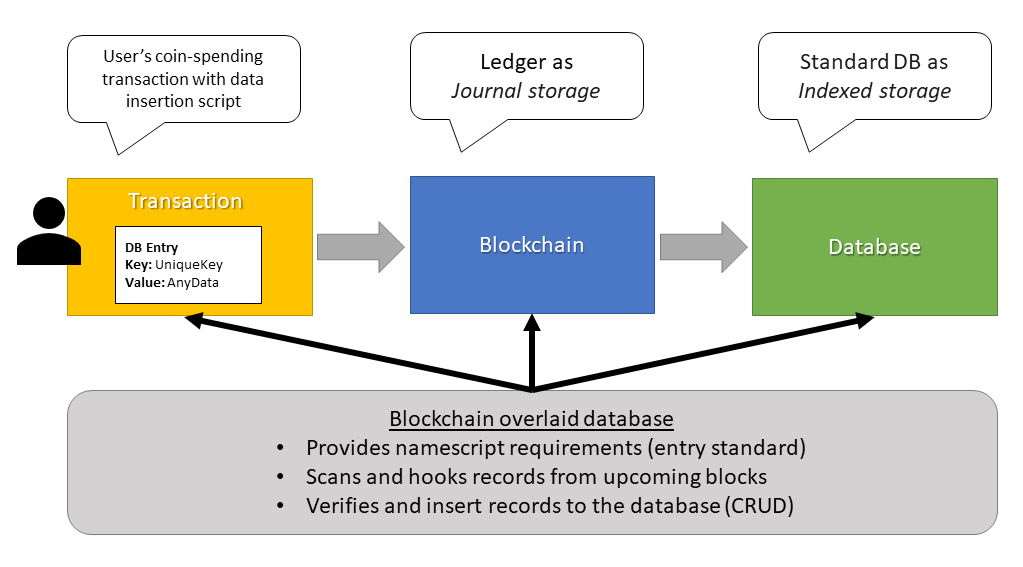
\includegraphics[scale=1.06]{src/Figures/chap1/chap1-fig02.jpg}
\caption{Relation of blockchain data to key-value database}\label{chap1-fig02}
\end{figure}

\begin{quote}
The system scans upcoming blocks according to the provided format standard and adds records to the database table. The entry may also contain the field which specifies till which block the entry is valid and some other data.
\end{quote}

In the first generation of DLTs (Bitcoin and similar), users apply specific scripts and methods to add arbitrary data in a coin transaction (from a few bytes up to around 100 kB per transaction including the transaction itself, i.e., in Bitcoin \cite{art1-key28}). As a result of such transaction, the coin itself is “burnt.”

In the second generation of DLTs, data insertion may have larger limits or no theoretical limits at all and are constrained by fees the user must pay for the message size. In Ethereum, for example, data insertion is performed by deploying a smart contract, which is designed as an application to store user’s arbitrary data. The combination of different types of ledgers in one bundle may require distinguishing common features and approaches, which will be reflected in the data format requirements.

\textbf{Data format.} To insert data, compliant with the cross-blockchain protocol, it must be structured in the following elements:
\begin{itemize}
\item \textit{“Key”} is a short string that identifies the user’s data; it must be unique across the bundle of blockchains. It is a searchable key in the database. In some systems it is also called “Name.”
\item \textit{“Value”} is any arbitrary data related to Key (Name).
\item \textit{“Lease time”} is a record which points out the number of a block, till the user’s key-value record will be valid. The outdated record will be erased from the database after this block. The initial record itself will be irrevocably stored in the blockchain where it has been published. This element is optional. But the developer should consider the constantly growing size of the database and can set up some defaults.
\end{itemize}

A key-value entry, or particularly an NVS record (as it is referred to Name-Value Storage technology), is attached to a user’s address in the result of a blockchain transaction, so this ensures the ownership of a record. Only the holder of the private key of the address may update or transfer the record; nobody else can publish the record with the same name while it is valid.

\textbf{Basic transactions.} There are three types of transactions: 

\begin{itemize}
\item \textbf{name new} – the creation of a new key-value record; before publishing, the record is checked with the database against its uniqueness; if the key already exists, the user may not publish it; though if the user did previously create it (the owner of the record), it can be updated;
\item \textbf{name update}, which includes
\begin{itemize}
\item[-] \textbf{value update} - the owner of the key can publish the same key, and add a new data in the field “Value;”
\item[-] \textbf{change Lease time} (reduce or extend); and 
\item[-] \textbf{transfer} key-value record to another address, and so transfer the ownership over this record; all these types of updates may be performed in the same transaction;
\end{itemize}
\item \textbf{name delete}-the owner publishes the name record with the instruction for deletion; from the block where it has been published, the records become invalid. The protocol passes the command to the database to erase the record. From the following block, any user may publish the same key again (because nobody owns it anymore).
\end{itemize}
\end{multicols}

\vspace{-.5cm}

\begin{figure}[H]
\centering
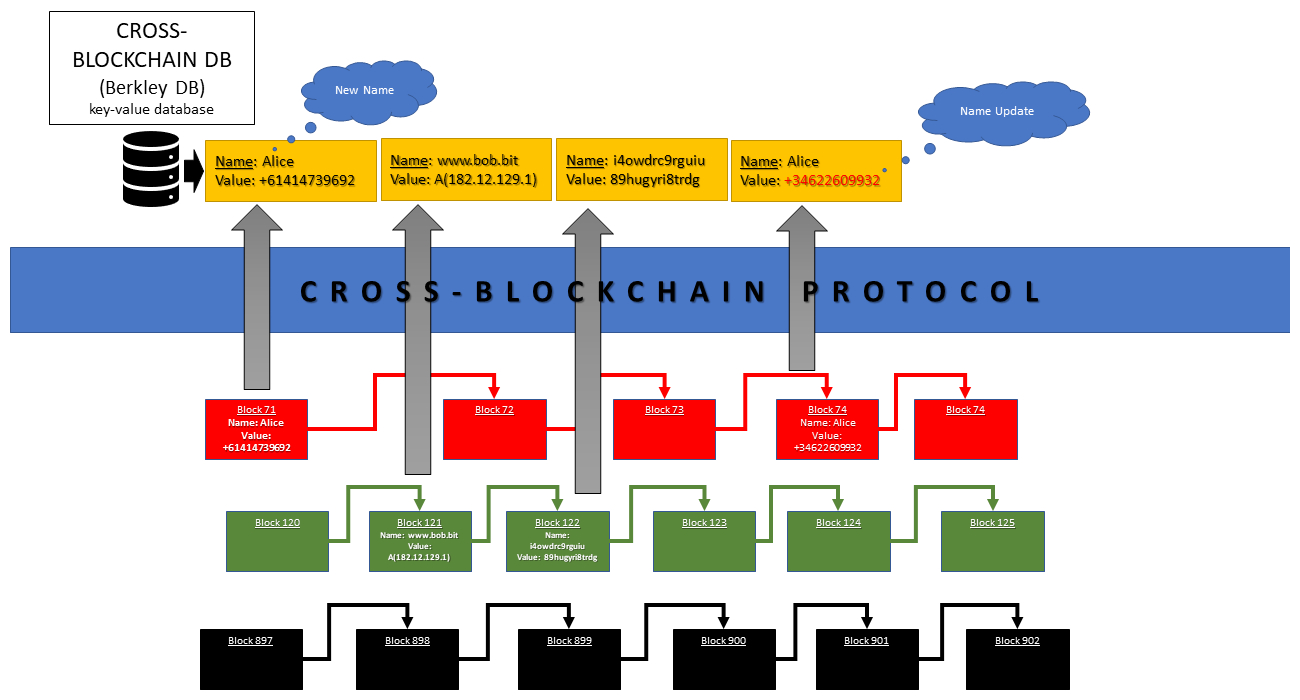
\includegraphics[scale=1.65]{src/Figures/chap1/chap1-fig03.jpg}
\caption{Cross-blockchain “key-value” database}\label{chap1-fig03}
\end{figure}

\begin{multicols}{2}

\vspace{-.6cm}

\begin{quote}
The scheme presents the bundle in dynamics. The system scans three ledgers: Redcoin (R), Greencoin (G), and Blackcoin (B). When it detects a complaint record, it hooks it up and adds to the overlaid database. The format is simplified; only Key and Value are traced. The hook detected blocks R-71, G-121, G-122 and R-74. Because R-74 contains the key from R-71, it updates the field Value in the relevant database record. 
\end{quote}

\vspace{-.4cm}
The concept of a database across a bundle of blockchains is presented in Figure~\ref{chap1-fig03}. The example of NVS in action is the following. The user publishes the key “Alice” and Value “+61414739692” to store the record of her public contact unless “Alice” already belongs to someone in the database. Anyone who enquires in their cross-blockchain node “Alice” will see the telephone number which belongs to a specific cryptocurrency address.

\vspace{-.1cm}

Timestamps provide the exclusiveness of keys in the database. Blockchain is a “timestamp machine,” which ensures certainty in the chronology of facts (transactions). 

\vspace{-.1cm}

The concept of blockchain timestamping is a matter of academic interest presented in several publications \cite{art1-key29}, \cite{art1-key30}, \cite{art1-key31}, \cite{art1-key32} and \cite{art1-key33}.

\vspace{-.1cm}

Thus, the Name which is published first in the bundle of blockchains appears in the cross-blockchain database, any other entries with the same keys are rejected; therefore, name squatting is impossible.

\vspace{-.1cm}

Key-value storage is a “raw material” for any sort of monetary and non-monetary tokens, overlaid digital currencies, smart contracts and decentralized applications.

\vspace{-.1cm}

From the perspective of any user, a cross-blockchain database is a public storage. Every user that installed the cross-blockchain protocol and full nodes (wallets) of every blockchain of the bundle will obtain a copy of such a public database.

When the user installs the nodes, the cross-blockchain protocol hooks key-value entries from downloading blocks.

When the user enquires a key, the system retrieves the information from the user’s local storage. Besides the decentralized nature of the database, another advantage is the high speed of interaction because the copy of the database is on the local machine.

We can summarize that the cross-blockchain protocol performs two main functions, i.e., input and output.

The \textbf{“Input”} mechanism is aimed to create a key-value complaint transaction, meaning that it must contain all required fields of a new database entry. The key itself must be unique in the database and must belong to one address, and the protocol accepts it only under this condition.

The \textbf{“Output”} tool scans downloading blocks and adds hooked records to the database file and responds to users’ queries to read entries from the database.

Any updates to database records are performed through blockchain transactions. It ensures that the user will not publish a key that already exists, will not capture someone’s key, and only the owner may publish updates and transfer it.

A standard wallet with integrated key-value storage should have UI and API, which provides necessary assistance for the user to create a correct key-value transaction for the cross-blockchain database.

Nevertheless, as far as public blockchain is an uncensored system, anyone may write manually the code of the transaction, which will not be necessarily compliant and send it directly to the mempool omitting the protocol. Therefore, a non-compliant entry will not appear as the record in the database. This is the major role of the output tool – to build a database as per the rules.

\setcounter{secnumdepth}{5}
\renewcommand\thesubsubsection{\arabic{section}.\arabic{subsection}.\alph{subsubsection}}
\vspace{-.2cm}

\subsection{Setting and Operation of the System}\label{subsec-4.2}

\vspace{-.3cm}

\subsubsection{How and which blockchain is to include in the bundle?}\label{subsubsec-4.2.a}

\vspace{-.3cm}

The cross-blockchain protocol is based on a social consensus, the same as any blockchain protocol at a higher level, is a social consensus: the one who agrees with rules provided by the blockchain protocol installs the node and run it.

\vspace{-.1cm}

In the architecture of a future cross-blockchain database, the first step is to define which blockchains are scanned, in other words, added in the bundle, and how to add and exclude blockchains. Typically, the user will download and install the same software, assuming that in this way the user expresses the consent.

\vspace{-.1cm}

At the same time, any other designed protocol may create an entirely different database using other lists of blockchains or the same blockchains but with other rules and filters.

\vspace{-.1cm}

It is also assumed that the provider of a rightful version of the national cross-blockchain protocol may be a government and therefore, it can be centralized to some extent. Furthermore, every user may decide to use multiple versions of protocols, including those provided by the government and or any other community.

\vspace{-.7cm}

\subsubsection{Initialization of a bundle}\label{subsubsec-4.2.b}

\vspace{-.3cm}

There are different types of blockchain protocols, and each may have different mechanisms of data insertion, which is discussed above. If the blockchain supports the Data Format and Basic Transactions described in the previous subsection, such blockchain can become a part of the bundle.

For better user experience, the blockchain wallet (node) should provide user-interface and API for data insertion complaint with the format and ensure that the user will not publish a key which already published by someone.

The criterion for choosing a blockchain to a bundle is reliability. Obviously, a PoW network with three nodes is less resistant to an attack then the network with three thousand nodes. As of today, there is no golden standard of blockchain security. Therefore, any decision must be empirically and expertly motivated.

\vspace{-.1cm}
The issue of network reliability is the subject of a separate study that is beyond the scope of this paper. However, for this work, we show which approach should be taken to automatically and independently diagnose the reliability.

\vspace{-.9cm}

\subsubsection{Exclusion of ledgers and rescue of names}\label{subsubsec-4.2.c}

\vspace{-.3cm}

The cross-blockchain protocol must be able to smoothly exclude on the run from the bundle any blockchain that becomes unreliable. The same action must be performed intendedly by all nodes of the system; otherwise, nodes will have different versions of their databases. 

\vspace{-.1cm}

The algorithms of exclusion and security criterion are defined during the initial set-up of the protocol.

\vspace{-.1cm}

The system should not receive metrics that trigger the exclusion from any third-party source, except the blockchains themselves since we strive for decentralization as the fundamental criterion of reliability.

\vspace{-.1cm}

However, in the following section certain centralized scenarios are also explained. 

\vspace{-.1cm}

A decentralized system works as follows. Each cross-blockchain node collects data from included blockchains for analysis. A blockchain network is indexed in the bundle while it meets the security threshold. Eventually, any running node will locally calculate these parameters and automatically exclude the network from indexing. Hence, every cross-blockchain node will apply the same algorithm, and it will end up with the same copy of the database across the bundle.

For PoW, this parameter can be difficulty/hash rate, number of nodes. For PoS, such parameter is PoS difficulty, among others. However, the security level is never enough, and there is plenty of room for further research and development.

When the cross-blockchain node detects a threat, it stops indexing jeopardized blockchain from the relevant block.

It is important to note that this exclusion happens not in the case of a hardfork and a roll-back attack (hardfork with rewriting the history deeper than the typical wait of confirmations), these issues are discussed in the next subsection.

After the exclusion of a blockchain, all records till the block of exclusion remain valid in the database and are available for reading. However, they are not admitted to normal transactions, i.e., name update and name delete become impossible. The user of the dropped blockchain can transfer the name from this blockchain to any other blockchain of the bundle.

The proposed concept of security leaves space for designing systems with different parameters. Here is one example. The bundle includes a few blockchains which have PoW and PoW+PoS consensus. The criteria for reliability for PoS and PoW are their dynamics of difficulty. If average difficulty decreases, say twice, nodes drop such blockchain. The difficulty is calculated periodically for each blockchain of the bundle, taking the longest period of difficult recalculation among blockchains in the bundle. For example, in Bitcoin, difficulty is recalculated every 2016 blocks (approximately two weeks), in Ethereum, it is dynamically recalculated so that on average, one block is produced by the entire network every 12 seconds \cite{art1-key34}.

\vspace{-.7cm}

\subsubsection{Adding on the run}\label{subsubsec-4.2.d}

\vspace{-.3cm}

Once chosen and built, the cross-blockchain system may require adding blockchains in the future. The main issue here is choosing the block to begin indexing from. This question is also relevant to initiating any new cross-blockchain protocol: from which block to start scanning if the blockchain is not new.

\vspace{-.1cm}

When a blockchain (which is running a while) is added in the bundle, rebuilding a database from the very first block may lead to a logic conflict with ownership. If in the added blockchain, one of the record already exists but was created earlier than the one in the current cross-blockchain database, a new re-indexed version of the database will re-assign this record. Thus, the owner of the record will lose control over it in the new database.

\vspace{-.1cm}

A better approach is to index a blockchain from the current block when it is being added. Hence, the reallocation of ownership is excluded.

\vspace{-.7cm}

\subsubsection{How to transfer a name between blockchains}\label{subsubsec-4.2.e}

\vspace{-.4cm}

The name record can be transferred from the dropped blockchain. For better user experience and competition between existing blockchains, the user should have this transferability also in running blockchains.

\vspace{-.1cm}

A user of a blockchain may transfer the record to any blockchain in the bundle. The user signs the string [record key + challenge] with their private key from the dropped network and then publishes this key in another blockchain. The system will see that someone is trying to capture the record, which already exists in the database. It will verify the digital signature, and if it belongs to the original owner of the record in the dropped blockchain, it will update the entry in the database.

\vspace{-.15cm}

The “challenge” is needed to exclude attempts of non-authorized capture of records. The owner could sign the key in the past for various reasons. Thus, the attacker could obtain the signature to reuse it. To exclude this, the owner signs the key with the ID of the latest block:

\vspace{-.4cm}

\begin{center}
\texttt{priv\_key(record\_key, latest block ID)}
\end{center}

\vspace{-.45cm}

Transferability of assets between blockchains is one of the most fundamental ideas of the cross-blockchain protocol because it supports competition between blockchains, which inevitably leads to a better quality of technology and services.

\vspace{-.6cm}

\subsubsection{Local Name-Value Storage vs. Cross-blockchain}\label{subsubsec-4.2.f}

\vspace{-.3cm}

Another issue of better design is the relation of a local and cross-blockchain key-value storage.

\vspace{-.1cm}

Any blockchain may have its own key-value storage even before it becomes a part of a cross-blockchain protocol. For example, Namecoin has NVS database to run TLD (Top-Level Domain) $^\ast$.bit, Emercoin runs NVS as a public database for general purposes and also maintains four TLDs (.coin, .emc, .lib, .bazar).

\vspace{-.1cm}

It is possible that names in one blockchain, when added to a global bundle, may conflict with other blockchains. Therefore, it is better for the design of the system that the local NVS running in parallel with the cross-blockchain database will prevent (or at least notify users) from publishing conflicting records.

\vspace{-.7cm}

\subsubsection{Name squatting protection}\label{subsubsec-4.2.g}

\vspace{-.3cm}

Namecoin designed the squatting protection for their system. When the user publishes a Name (key), it becomes available publicly in the mempool before publishing in the blockchain. In PoW, users can compete for the priority of a transaction by proposing miners a higher fee. The attacker right after has seen the name in the mempool can try to push the same name first by proposing a higher fee, and so to capture it.

\vspace{-.1cm}

For that reason, Namecoin designed a two-step publishing protocol \cite{art1-key35}: (1) publish the hash of the name; then (2) publish the name itself.

\vspace{-.15cm}

In Emercoin, the queue is ordered chronologically, and fees even though are proposed they are burned instead, the miner/minter gets no fee from the user.

\vspace{-.15cm}

Cross-blockchain must be designed in the way to accommodate both models. For blockchains, where easy squatting is possible, there should be two steps.

\vspace{-.15cm}

When the squatter is a miner (minter), there is no simple solution though, because the miner may shuffle the queue. However, if the system design does not allow cheating, squatting is just a free-market competition of who registers the name first. It is recommended to use two-step protocol in all cases, propose higher fees and publish a new name simultaneously in all blockchains of the bundle; it reduces the chances for a squatter to capture the name. Once a new name is published, its capture in further transactions is impossible.

\vspace{-.9cm}

\subsubsection{Database}\label{subsubsec-4.2.h}

\vspace{-.3cm}

The choice of appropriate technology for the database is an essential step in designing the cross-blockchain system. Obviously, it may be unreasonable to create from scratch a new technology for the database; the market proposes an extensive choice of reliable solutions.

\vspace{-.1cm}

Under the hood of Emercoin’s Name-Value Storage is Berkeley DB \cite{art1-key36}, an Oracle’s key-value database. Initially, many elements of the Bitcoin system relied heavily on Berkeley DB. Subsequently, in version 0.8.1, developers migrated to LevelDB \cite{art1-key37} to store transactions and block indices but left “wallet.dat” on Berkley DB \cite{art1-key38}. 

\vspace{-.1cm}

There might be reasons to choose one or another solution (LevelDB, Redis, among others) or a database from SQL family, depending on the needs of the specific project. Worth noting that the database is the fundamental of software.

\vspace{-.1cm}

Furthermore, since we create the cross-blockchain database for applications, the choice of the database should match the needs of further development.

\vspace{-.1cm}

A high-level design concept is presented in Figure~\ref{chap1-fig04}.
\begin{figure}[H]
\centering
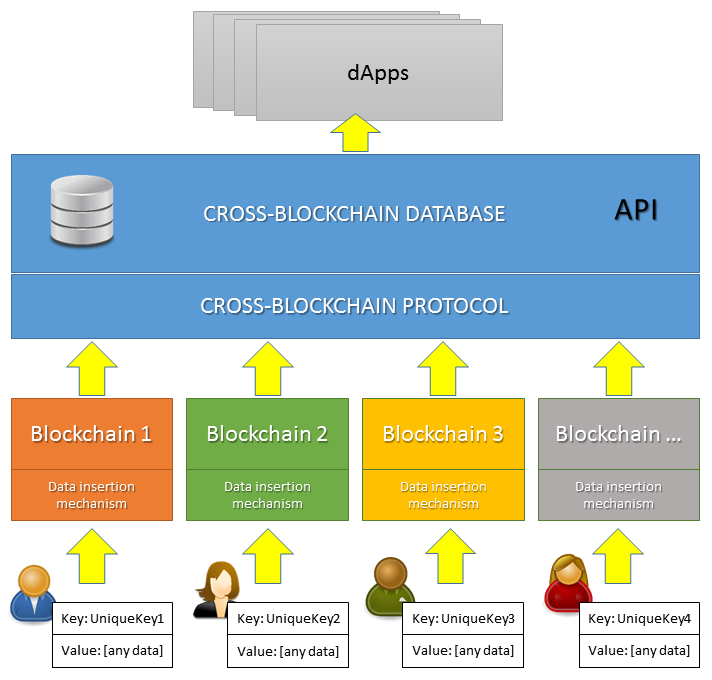
\includegraphics[scale=1.38]{src/Figures/chap1/chap1-fig04.jpg}
\caption{Cross-blockchain protocol scheme}\label{chap1-fig04}
\end{figure}

\begin{quote}
The scheme presents a more general scheme of the bundle interaction. Users may choose any ledger in the bundle to publish records. The protocol creates a database of user’s entries across these ledgers. The database is used to develop decentralized applications. 
\end{quote}

\vspace{-.35cm}

Blockchains towards the database play the role of the channel through which users insert and manage data.
 
Cross-blockchain database has CRUD features, but because they are performed through blockchains, delete and update in blockchains themselves is impossible. They are immutable logs through which CRUD commands are passed and performed in the database.

The second important role of the blockchain is a mechanism of ownership because records are attached to the addresses of their users. Through the native blockchain mechanism of addresses and private keys, database records are managed and transferred between users as tokens.

The cross-blockchain protocol ensures the connection of blockchains in the bundle with the database.

To make sure the record gets into the database, data insertion accompanied with protocol format, for instance, key-value record entries will require the user to fill in the relevant fields, and other requirements of the designed format.

Then system checks against the database the uniqueness of the key; if the key exists in the database, the system ensures that only the owner of the address may publish an update. If the rules are followed, the entry is packed in the blockchain transaction and published in the chosen blockchain.

In the result of data insertion in the blockchain, the entry gets into the database. It makes no sense for the user to change or somehow omit the algorithms of the protocol in their local machine, trying to publish the name that someone already owns. Even the user makes this trick pushing the name up to the database, this version of the database will exist only on the user’s machine, while all other cross-blockchain nodes will have the normal version. This is a mechanism of a social consensus, i.e., users install the protocol, resulting in the same local copy of the database.

The database may be used for developing various user applications. Since DB is local, the interaction is instant, which makes possible development of heavily loaded applications.

\subsection{How to chronologize the index}\label{subsec-4.3}

\vspace{-.2cm}

This section discusses the problem of the inaccuracy of time in blockchains compared to each other and astronomical time, the possible consequences of hardforks, and roll-back attacks and variants of the system design to address these issues.

\vspace{-.6cm}

\subsubsection{Inherent issues of blockchain to deal with in the bundle architecture}\label{subsubsec-4.3.a}

Let us define and evaluate issues to deal with in a cross-blockchain architecture.

\textit{Mistiming}. Timestamps in each blockchain are not necessarily accurate to astronomical time. It happens because a node which closes a block includes a timestamp based on its knowledge of current time, which might be inaccurate. Usually, two protocol limits are applied here: a block cannot be earlier than the last block and 2 hours ahead from the median time of network peers. This rule is relevant to Bitcoin and many other similar systems, though these parameters are specific to a block platform \cite{art1-key39}. 

\textit{Orphan blocks}. The longest chain of blocks is accepted, and shorter is dropped out. Nodes compete for finding new blocks, and this kind of fork happens each time whenever any node presents the network a correct longer chain. If not addressed in the design of the system, it will create the problem of a forked database because the cross-blockchain protocol does not re-index the whole ledger when a new block arrives.

\textit{Hardfork}. Let us separate a retroactive “roll-back” attack in another category. Here we consider a hardfork that is not a result of the attack, but a conscious and willing decision to change the blockchain protocol. The nodes that did not switch to a newer protocol will see incompatible blocks which will not be able to accept. The minority may create their network by forking. Two versions of the blockchain will have the same history of blocks till the block of the split. After that, users will have the same amount of cryptocurrency, the same tokens and smart contracts in both networks. The protocol will not know about the parallel network. That is a solution itself, however. Nevertheless, it is assumed that the community may wish to include the fork to the bundle. Is an automatic inclusion of a forked network for indexing possible? The solution must address the problem of logic collisions when two records in different blockchains represent the same asset.

\textit{Retroactivity (roll-back)}. Even though some DLT systems may be designed to allow retroactivity as a legitimate feature, we assume that the immutability must be preserved as the major advantage. Therefore, we consider a roll-back as a form of attack which can cause a hardfork of the database in the cross-blockchain bundle. The running node will not notice a history change because it does not re-index from the beginning of the database each time a new block arrives. If the record belonged to address A in the original blockchain, and in the result of retroactivity, it was re-assigned to address B, the database will still contain the record of the entry attached to address A. At the same time, when a new node is installed, or the old node starts re-indexing, it will create a new database file with the key attached to address B. Therefore, new and re-indexed nodes will have a forked version of the database, while old nodes will have the original one.

Let us discuss possible solutions and evaluate their applicability.

\vspace{-.3cm}

\subsubsection{Assumption of time inaccuracy}\label{subsubsec-4.3.b}

\vspace{-.5cm}

Inaccuracy may create some negative user experience. For instance, in green blockchain (see Figure~\ref{chap1-fig05}), the miner finalizes the block with the timestamp that is 02:12 ahead of the current astronomical time. In red blockchain, the block is closed 19 seconds earlier astronomical time. If the same records are published there, they will be accepted only from the red blockchain, even though they are published at the same astronomical time. Technically, even though they happened simultaneously according to the astronomical time, the red one will be earlier, which is compliant with the protocol.
\end{multicols}
\begin{figure}[H]
\centering
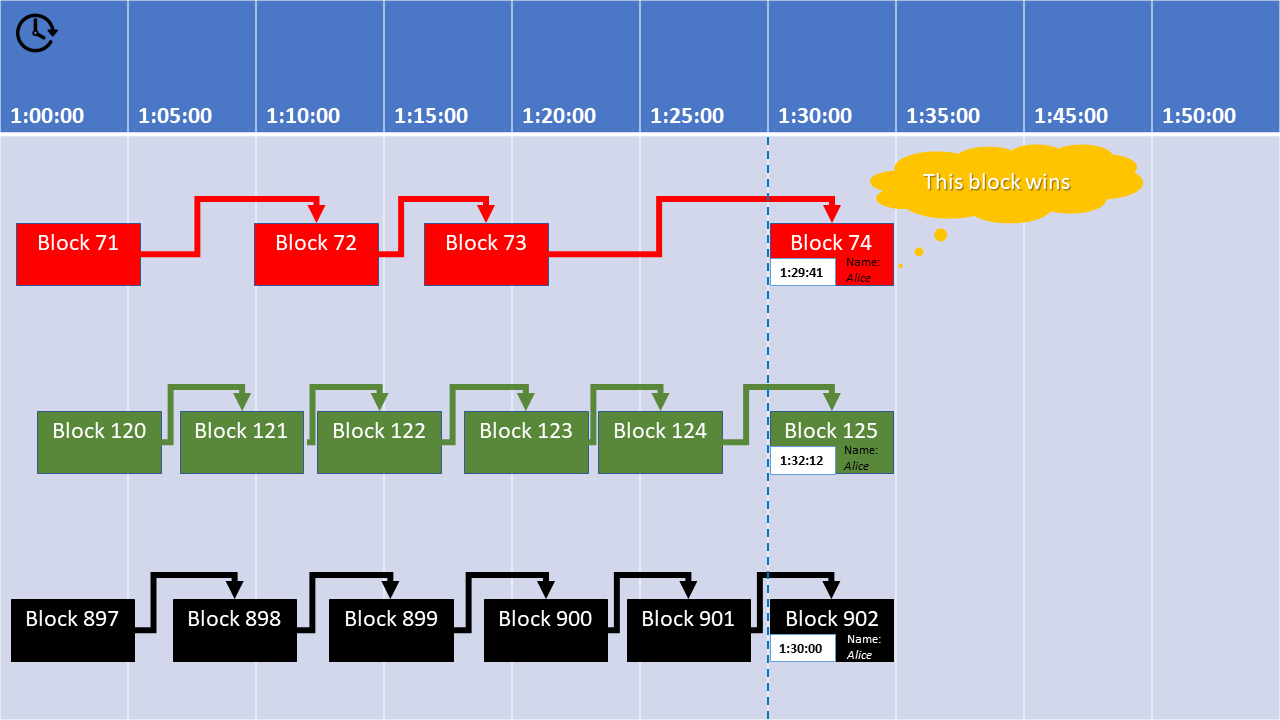
\includegraphics[scale=1.71]{src/Figures/chap1/chap1-fig05.jpg}
\caption{Mistiming of key publication}\label{chap1-fig05}
\end{figure}

\begin{multicols}{2}
\begin{quote}
Three transactions happened simultaneously as per the astronomical time, at 1:30, but each network has time discrepancy; therefore, the red chain is taken first (19 seconds earlier)
\end{quote}

Publication of the key at the same time can also be an issue. However, even if it happens, the node will compare timestamps of transactions in blocks and will select the one which is earlier among the blocks.

Time inaccuracy is a natural limit that cannot be resolved in a cross-blockchain index without either centralization or changing the protocol of each blockchain to provide for cross-blockchain time synchronization. Because such changes require hardforks in existing blockchains, they may become infeasible due to their decentralized nature.

Therefore, it is proposed that time inaccuracy will be the assumption users must accept. Free market competition will demand blockchain communities to provide for better services and user experience. If the record is valuable, the user may wish to send the same key simultaneously for the registration in all blockchains of the bundle, thus competing with themselves. Once one transaction arrives first in one of the blockchains, the user may wish to transfer it to that blockchain where they want to manage it.

\setcounter{secnumdepth}{5}
\renewcommand\thesubsubsection{\arabic{section}.\arabic{subsection}.\alph{subsubsection}}

\vspace{-.6cm}

\subsubsection{Orphan blocks}\label{subsubsec-4.3.c}

\vspace{-.4cm}

The cross-blockchain protocol solves the problem of orphan blocks by pending a few blocks after the record was published. In general, this period is called “confirmations,” and it is specific for different consensus; for example, in Bitcoin, 6-blocks are the reasonable time that reduces the probability of the fork \cite{art1-key40}.

Therefore, in the cross-blockchain system, each blockchain will have its own pending time, and the protocol is tasked to add records to the cross-blockchain database after this quarantine.

\vspace{-.6cm}

\subsubsection{Hardforks}\label{subsubsec-4.3.d}

\vspace{-.4cm}

Hardforks are different from just orphan blocks due to how they create two sustainable independent networks. One will be the majority, and users will typically see this branch of the network. If the minority is organized enough, they may establish a new network. Till the block of the hardfork, two networks have the same blockchain history. However, from the next block after the fork, all assets can be independently moved within the new blockchain, thereby creating a kind of double-spending.

To address this issue, let us define the scenarios of a hardfork.

\begin{itemize}
\item[(1)] The majority of nodes do not change the current protocol, only the minority buds off with a new protocol incompatible with the current. In this case, it is not necessary to do anything. The fork will exist as Elusive Joe; unless the mainstream community wishes to include it in the bundle.
\item[(2)] Inclusion of a minor fork may happen in the following way. Beforehand the hardfork miners will put flags in blocks for the future fork, announcing to the community the number of the block from which the fork will happen. The protocol detecting the threshold of flags (say, 10\% of nodes) will require the user to explicitly include this blockchain as a new one in the bundle.
\item[(3)] To resolve the issue of duplicating keys, the protocol will apply the following rule. Until the user does not make any transaction in the bundle, doubled keys do not constitute a problem itself; they can exist in parallel at any length of time. The user may decide to transfer the record or update it in any of the blockchains. The transaction which happens first among two blockchains will be accepted in the protocol, and from that moment, any other transaction in the parallel blockchain will never be approved by the protocol.
\item[(4)] In the case when the majority is going to move to another protocol, the community will also use flags. When the system detects that the majority is going to adapt an incompatible protocol, the protocol will stop indexing the blockchain, and then ask the user for explicit consent for the new version of the blockchain in the bundle. This scenario can be combined with the accommodation of both blockchains described in (2) and (3).
\end{itemize}

In both cases with flags, the system requires the user’s consent; otherwise, the protocol stops running the bundle in the user’s machine, thereby preventing the cross-blockchain database forking.

\vspace{-.5cm}

\subsubsection{Retroactivity}\label{subsubsec-4.3.e}

\vspace{-.3cm}

Retroactivity can cause the reallocation of ownership of NVS records in the blockchain locally, as well as capturing records from other blockchains of the bundle.

There are two specific issues to address:
\begin{itemize}
\item[(1)] The node does not know on the run of a deep reorganization of blocks in the blockchain. Technically, this is still a legitimate behavior. Here, it applies the rule of the longest chain of blocks. When it is presented to the network, nodes automatically pick it up, replacing the current chain. Because the cross-blockchain system does not re-index database, changes in ownership that happened due to this attack will not be reflected. That might be though as a solution itself; but
\item[(2)] When a new bundle is installed, or the same bundle is re-indexed from the very beginning, the resulting database will reflect changes that have happened due to the attack.
\end{itemize}

Therefore, in the result of retroactivity, some users of the community will have one version, some users another.

Before discussing the possible solutions, let us define the probability of this attack.

The fault tolerance of the bundle is defined by multiplication of probabilities of the attack of all blockchains of the bundle, because the failure of at least one blockchain in the group may lead to the failure of the whole bundle:
\begin{equation}
P=(1-(1-p_{1})(1-p_{2})(1-p_{\text{n}}))\label{equ1}
\end{equation}

The challenge is the practical part of this evaluation. The simple mathematical expectation of the attack for a bundle can be 0. Therefore, statistical methods may not be helpful.

Thus, we keep this in mind as a theory. For the implementation of any system based on this concept, it will be a good practice to remember that there are no perfect systems, and all reasonable measures must be put into consideration.

More important is not the level of resistance to attacks, but the ability of the system to restore after the fault. Thus, let us define some measures that can be designed to address possible retroactivity issues.

In principle, four actions must be taken: (1) the node must detect an attack; (2) the node must detach the fault blockchain from the bundle; (3) a new or re-indexed node, must define that there was an attack and be able to build an uncorrupted database across the bundle; (4) the node must support the transferability of records from the fault blockchain to any of blockchains in the bundle.

Here is the solution.
\begin{itemize}
\item[(a)] The running node will define retroactivity as a legitimate feature because here applies the rule of the longest chain. It is proposed to add heuristic analyzes at the level of the cross-blockchain protocol. It will keep the state of blockchain headers and compare them to detect changes that happen deeper than a normal reorganization of blocks (see “Orphan forks”).

For instance, for Bitcoin, the norm will be to change up 6 blocks in depth. For each blockchain, this figure will vary. When the system detects an abnormal fork, it defines the depth of the fork by comparing two states of headers and marks the blockchain excluded from this block and continues indexing other ledgers of the bundle. When the attack is detected, it also recommended to backup the database. An automatic backup must happen when a new version with the chain of blocks deeper then $n$‑blocks appears in the node. As a result of this step, the running system will preserve the original state of the database and will detach the fault blockchain from the further indexing and will continue working.

\item[(b)] To detect corruption when installing a new node/re-indexing, an approach of redundant copies can be used, similar to RAID massive, see Figure~\ref{chap1-fig06}. Existing methods for data storage among multiple drives are relevant to name-value storage. RAID has different methods. For example, in cross-blockchain protocol with RAID 1 \cite{art1-key41}, the user will store the name in two or more blockchains. If one blockchain is attacked, when re-indexing the system, the node will detect the collision at some block by analysis of RAID collisions.

\item[(c)] The publication of a RAID record must contain the signatures of the [record\_key+challenge] from the parallel blockchain. The pointer to the highest block will help to detect the exact height of the blockchain attack. From this moment, the system will detach the blockchain from indexing, allowing the possibility to rescue records from the fault blockchain by a transfer to rest in the bundle.
\end{itemize}
\begin{figure}[H]
\centering
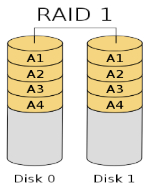
\includegraphics[scale=3]{src/Figures/chap1/chap1-fig06.jpg}
\caption{RAID 1}\label{chap1-fig06}
\end{figure}

\begin{quote}
Basic RAID 1 scheme with two storages where data is duplicated.
\end{quote}

Because the probability of a successful attack of two blockchains at the same time is significantly lower, RAID methods may create enough protection. The more redundancy, the lower are chances of the fault of the cross-blockchain database.

\section{Evaluation of the invention or why does the cross-blockchain\\ protocol suit governments?}\label{sec-5}

This section evaluates how the cross-blockchain protocol addresses the issues defined in Section 3 and corresponds with the initial goal to develop a system that suits government purposes, i.e., to run, for example, property registry using various public blockchains. It consists of two subsections: brief evaluation (\ref{subsec-5.1}) and extended discussion with scenarios (\ref{subsec-5.2}).

\subsection{Brief evaluation}\label{subsec-5.1}

Hardforks are addressed by filtering duplicate assets after a hardfork. The protocol must contain rules to define which record the user updates first after the hardfork. Hence, the duplicated record in the parallel system is not traced anymore.
 
Two complementary solutions address immutability and the ability to enforce lawful actions: records are validated by cross-references, and the protocol can be patched by trusted addresses.

Each of this element inside has various scenarios which are further discussed. Here are basic examples: Alice creates a record that represents her property rights (token), and in the token, she writes who validated it, literarily, who says that this token represents her property right, say, land title. Let it be Bob. Bob creates his key-value record, which says the world “Alice’s token is valid.” While Alice controls her private key, she can perform transactions with her asset. If Alice lost her key, she would ask Bob to update his record, that her token is not valid anymore, and re-issue a new token. 

Bob may also update record in case of her death, or based on a court decision, etc. One asset may have multiple references to such trusted third parties: land registry, notary, court, land surveyor, local government, building inspector, etc. Invalidation provided by any of these authorities may trigger some logic in the system. The logic itself must reflect legislative norms and government structure of the jurisdiction where this system is implemented. That is why this system is called “smart laws.”

The second level is an “emergency brake.” It is obvious that Bob is part of the government. Bob’s authority is validated hierarchically by someone higher, using the same method of cross-references. This system reflects a real-life public office, which has an appointment and dismissal procedure.

We eventually come to the root record, or multiple roots (because of separation of powers). If Bob [the authority] abuse power, the court, which is another authority that  has no interconnection with Bob’s root, may \textit{patch} the protocol.

Root address(es) must be pre-installed in the user’s system. Each root record may have its specific role and power, i.e., an authorization of what it can do and what cannot.

Therefore, the court publishes the record, which says the system “Bob’s authority is invalid.” The court may also publish a new rule for Alice’s token. Because the user’s node trusts the court’s address, it hooks this patch and applies new rules. In this way, Alice token, if stolen, will be invalidated. Bob will lose its authority. Of course, this is a simple example; the system may contain addresses which are managed collectively (multi signatures), it is possible that in the future the system will have e-voting (e-referendum) mechanisms directly on blockchain. There is still a possible solution when the government announces off-chain (for example, by publishing in Gazette) which address (root) is valid/invalid. And finally, each person leaves the right to exclude the “root” if he or she does not trust the government anymore.

The advantage of such system is that all records, including patches, remain irrevocable at the level of blockchains. Any digital dictatorship can eventually be thrown, and all blocks rescanned from the beginning with new fair rules and filters which rebuild the database, so Bob will get his authority back, even though there is still somewhere in the ledger the record that claimed his address invalid.

To address the issue of digital identity is it proposed a similar way of cross-referencing. Alice creates her token that says she is Alice, Dave (trust service provider), creates his token where he says Alice’s digital identity is valid. To address the issue of privacy, it is proposed not to publish any personal data on-chain. Various methods and frameworks may be applied (see the next subsection) to publish only cryptographic fingerprints but to store personal data off-chain.

The cross-blockchain protocol addresses the problem of scalability and price volatility. The bundle of blockchains together can have a good performance. Not the government decides which blockchain to use but the user. The user can also transfer the asset from one ledger to another within the bundle. These mechanisms leverage fair market competition of technologies and services. Even if at some point in time one ledger is overloaded with transactions, fees will rise in this blockchain. Unsatisfied users will choose other ledgers in the bundle, with better performance and suitable fees.

\subsection{Why does the cross-blockchain protocol suit governments?}\label{subsec-5.2}

\setcounter{secnumdepth}{5}
\renewcommand\thesubsubsection{\arabic{section}.\arabic{subsection}.\alph{subsubsection}}

\subsubsection{Hardforks}\label{subsubsec-5.2.a}

Nowadays, the government plays the role of a keeper of property registries. In different countries, they may have different names and specializations (cadastre, land title registry, real estate registry, among others). Still, the purpose is the same: to provide certainty in property rights by tracking records of transactions (title deeds). Besides land titles, there are registries for movable properties (cars, boats, aircraft, etc.), shares, and other securities and corporate rights.

The use of any decentralized system, including the blockchain, was limited because it could create issues with registry forking. The solution of having one blockchain and the government will point out which is legitimate, for example, Bitcoin or Bitcoin Cash, Ethereum or Ethereum Classic, is unlikely to be acceptable. Why would anyone use a decentralized system but end-up with the central authority? It disables competition between blockchains.

The cross-blockchain protocol addresses it with a free choice for users. The proposed protocol may support both blockchains after their fork. The same as Schrödinger’s cat, the record has a dual nature until the user chooses. Having two records is not a legal collision; it becomes so when the user performs two different transactions with the same record in different blockchains of the bundle. Therefore, the protocol ensures that a user’s choice is irrevocable. Once it is done, they will not be able to perform a conflicting transaction in the second blockchain. Therefore, hardfork is not a problem anymore.

\subsubsection{Immutability, trusted third parties and\\ governance}\label{subsubsec-5.2.b}

\vspace{-.2cm}

Blockchain immutability is considered as one of the major advantages of blockchain technology. The transaction records and inserted data are irrevocable and immutable. Since the blockchain was invented, the discussion of its use for state governance is opened, especially towards property registries.

In the previous subsections, we discussed the example when the key-value record represents someone’s property rights, for instance, the land title.

The record itself worth nothing unless there is a certainty that it has a legal connection with the real-world asset. With the cross-blockchain database, it is possible to create an ecosystem of trust, where records refer to other records certifying them.

For example, Alice publishes her land title record. Bob, a town clerk, creates his record where he certifies that Alice’s record duly represents her land title (see Figure~\ref{chap1-fig07}).
\end{multicols}

\begin{figure}[H]
\centering
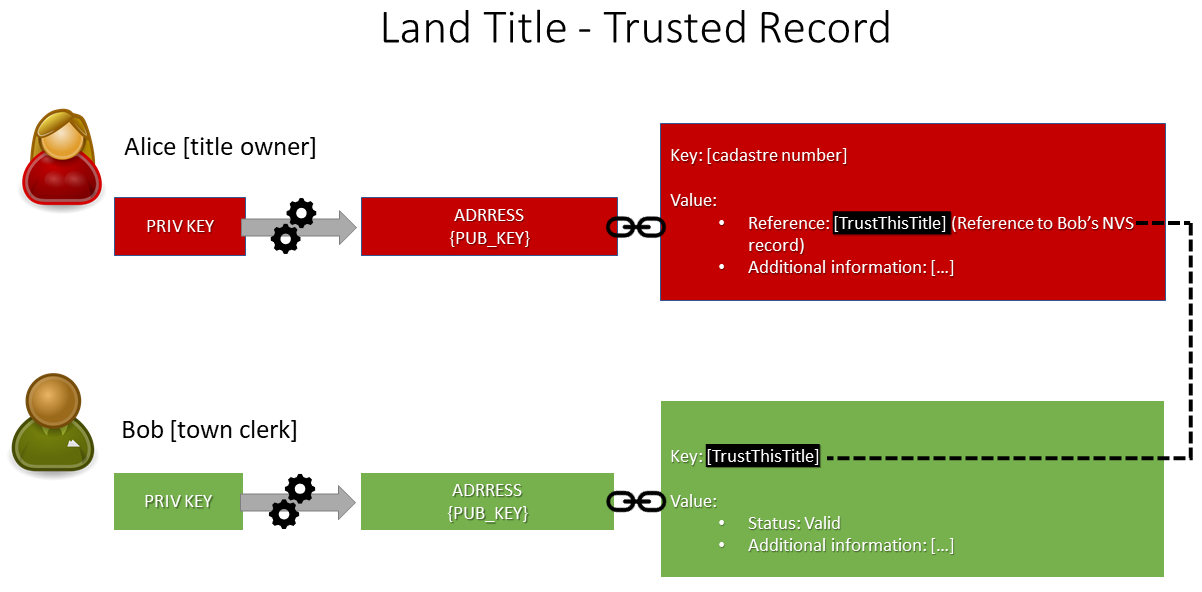
\includegraphics[scale=1.8]{src/Figures/chap1/chap1-fig07.jpg}
\caption{Scheme of trust services}\label{chap1-fig07}
\end{figure}

\begin{multicols}{2}
\begin{quote}
Alice included in Value the reference to Bob’s record with the key “TrustThisTitle” (read, any valid key). Bob’s record says that Alice’s record is valid. Alice used Redcoin, Bob - Greencoin. Because they are in the bundle, the system may resolve an inquiry on the validity of Alice’s token. It searches in the database the key [cadastral number], parses it to find a reference. When the reference [TrustThisTitle] is found, the system searches it as the key to the database entry. When [TrustThisTitle] entry is found, it parses its value to find the status “valid.” Because we trust Bob, he is our town clerk, we trust Alice’s record that represents her property right. Land title used here as an example. Any property rights and facts can be certified.
\end{quote}

To buy Alice’s land, Charles needs to acquire her record. Charles will enquire Alice’s record in the cross-blockchain database and will find in this record the reference to Bob’s record. The system will enquire Bob’s statement, which certifies Alice’s asset. Charles trusts Bob; hence, Charles can trust Alice’s record and make a title deed even without meeting her in person. The parties may do an atomic swap: Alice will send him the title record, and Charles will pay cryptocurrency in return.

In this way, any real-world facts can be certified: immovable and movable property, digital identity, facts of life (birth, death, missing, etc.), contracts, for instance, acknowledgment by a notary public (for civil law countries), facts of some events (force majeure, etc.). See Figure~\ref{chap1-fig08}.
\begin{figure}[H]
\centering
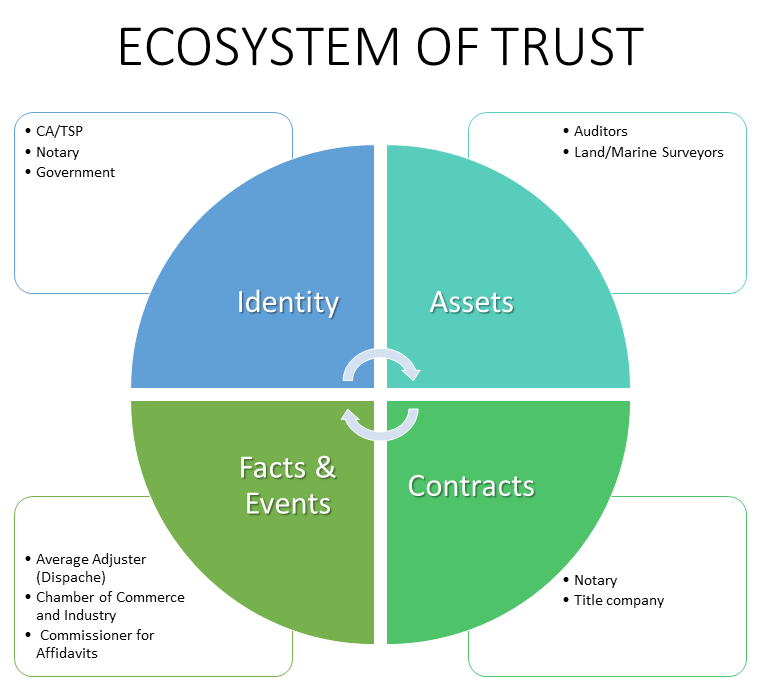
\includegraphics[scale=1.35]{src/Figures/chap1/chap1-fig08.jpg}
\caption{Map of trust records and trust providers}\label{chap1-fig08}
\end{figure}

\begin{quote}
The map shows examples of how third parties in real-world cases certify identity, assets, contracts, and facts \& events: Identity by Certificate Authorities or Trust Service Providers (EU), by a notary public and different government agencies. Assets are verified by auditors, land and marine surveyors. Contracts can be certified by notaries, land title deeds by title companies. Facts and events by Dispache (a person who certifies claims, especially for marine insurance), by Chamber of Commerce and Industry the origin of products and force majore events, Commissioner for Affidavits certifies witnesses declarations and statements. 
\end{quote}

Obviously, it is impossible to completely get rid of trusted third parties, at least at this level of science and technology. Trust records address the problem of credibility. An intermediary is a “necessary evil,” especially in the world of growing digitalization and remote relationships.

Without commercial intermediaries and governments, relations would have looked like scenes from gangster movies where the seller and the buyer need to meet personally and show each other the money and the product to make the deal. The progress required more effective economic forms. According to Potts et al. \cite{art1-key42}, the current U.S. GPD consists of 33\% of services produced by intermediaries.

In the proposed scheme, if Alice lost her private key, she cannot sell her property anymore. She may ask Bob to update his record specifying that Alice’s record is not valid anymore.

\textbf{Digital identity.} Likewise, a conventional Public Key Infrastructure (PKI), the cross-blockchain database can be used to store certificates of digital identity. At the government level, there can be a root record, which will enable multilevel hierarchical trust interaction. For example, if Alice’s and Bob’s keys are compromised at the same time, Bob’s upper validator will mark his record invalid, and so on, going up to the root record if needed.

The scheme also accommodates two/multi-factor authorization (2FA/MFA) and hardware devices for signing transactions, for instance, hardware crypto wallets.

For 2FA/MFA, Alice will ask a trusted third party to send a “challenge” (secret phrase) using a closed trusted channel established during initial identification, which she will sign and include in the transaction as proof. The trust provider, at the same time, will publish the hash of the secret in the cross-blockchain database\footnote{This is one of many possible 2FA/MFA protocols as an example.}.

To protect the private key from a theft, Alice will use a hardware wallet. For example, in the EU, such a level of protection is necessary to have a non-reputable\footnote{A signature for which the signatory cannot deny that they are the originator of such a signature (as per eIDAS regulation in the EU).} Qualified Electronic Signature, as per eIDAS regulation \cite{art1-key43}.

The government may keep the “root” of trust, the record which is used to sign certificates of trusted third parties, also known as “Certificate Authorities” and more specifically for eIDAS “Trust Service Providers.”

Such identity and trust services, even though they require third parties, are not necessarily highly centralized. Opposite to a single root record, there can be multiple roots and self-signed certificates of numerous third parties. Alice as an end-user decides whom she trusts creating her white list of credible entities, including government root, commercial providers, or even her circle, similar to the concept of “web-of-trust” \cite{art1-key44}: Alice trusts Bob, but does not know Charles, Bob trusts Charles, therefore, Alice trusts Charles. See Figure~\ref{chap1-fig09}.
\begin{figure}[H]
\centering
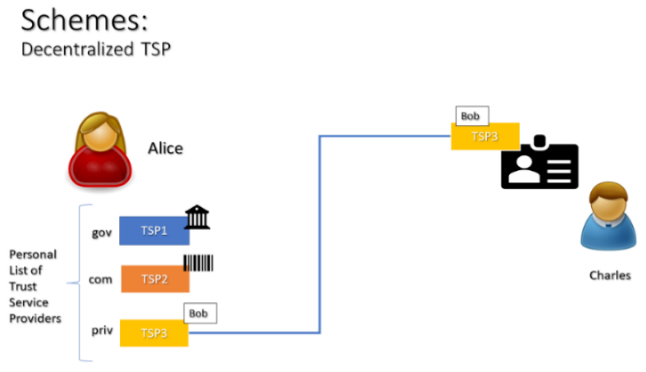
\includegraphics[scale=1.65]{src/Figures/chap1/chap1-fig09.jpg}
\caption{Multiple TSP providers}\label{chap1-fig09}
\end{figure}

\begin{quote}
In a decentralized trust scheme, Alice can create her list of trusted addresses that belong to the government, a commercial trust service provider and Bob (web-of-trust scheme). Because she trusts Bob and Bob certified Charles’s digital identity, Alice can trust Charles, even without knowing and meeting him personally.
\end{quote}

The source of truth is in the sequence of published key-value records where the latest record represents the current state of affairs (valid, invalid, revoked, compromised, stolen, etc.). This is the first level of overcoming the immutability where the blockchain plays an important role because no record can be voluntarily altered or erased, and all the history of transactions is preserved.

\textbf{Jurisdiction as a filter.} However, what if the root is compromised? To address this issue, the system will use patches.

The bundle’s output mechanism can be considered as a filter. In the discussion above, we proposed “timestamp” as the main rule for filtering records. The bundle ignores repeating entries, adding to the database only first found unique keys and then tracks updates to these records.

If we look at any jurisdiction as a kind of filter, the laws will be these filtering rules. What we normally call “legal” (as per the law) is not filtered in the system and shown in the database. In this way, legal norms and procedures can be digitized and applied to transactions.

The smart laws in the cross-blockchain protocol are the rules which have at least two elements:
\begin{itemize}
\item[(1)] Cross-references, when one record (authority) validates another record (asset, digital identity, fact or contract), this level does not influence the database records; it is a logic how to resolve queries to records based on their references in the database; and
\item[(2)] At least one trusted root address initiated in the bundle as a “digital authority,” which may publish records in a ledger that are considered in the system as \textit{protocol patches}. The patch will contain a command (a new rule) for the database; the system will apply the patch to update the database by: deleting existing records, including the record which exists at the level of a ledger but not included in the database or ignores some address.
\end{itemize}

Both elements can be much more complicated based on the existing intricacies of political system and regulations.

If the root record is compromised, the cross-blockchain authority must reset the trust using one of the proposed scenarios:
\begin{itemize}
\item[-] Distributed (social consensus) – users will arbitrarily install root address(es) and accept patches; though it may lead to multiple hardforks of the cross-blockchain database, different communities which stick to different roots will see a different state of affairs in the database;
\item[-] Centralized – patches are published from the trusted address (or addresses), initially provided in the system, the patch is automatically recognized as authorized instructions and installed by the system, but if the root is compromised the authority announces it invalid off-chain. Users to have a legitimate version of the database will have to install a new root address and reindex the bundle. Normally, users will download a new version of the cross-blockchain software from the official web-site;
\item[-] De-centralized (collective control over the root address) – The patch is initially created in the system, with a blank Value, and controlled by a multi-signature scheme. A user’s system accepts updates of the field Value where patches are published based on a collective decision in the multi-signature scheme.
\end{itemize}

It is considered that in the future, direct e-voting on the blockchain with automatic implementation may also be designed to address the issue of decentralized governance in large-scaled online systems. The combination of these methods can make the system more sustainable.

\vspace{-.1cm}

Also, many other cases are possible in a “smart law.” For instance, Alice died, and Charles has the right to inherit her record. When Alice designed her “smart will,” she could not know which notary would fulfill her will, even if she specifies all licensed notaries in the country, by the time of her death, it might appear a notary cannot execute the smart will because the list is invalid anymore, for example, because of the root reset. Hence, none notary has access to trigger the “smart” inheritance.

\vspace{-.1cm}

In traditional “paper” bureaucracy, Charles will apply to any notary to issue a record of inheritance that grants him Alice’s title right; the only thing that matters here is that, by the time of application, he has to choose one of the existing authorized notaries. Even if Alice designed her will to perform execution automatically without any notary, this similar issue would still arise. Who will certify her death to trigger self-execution of the will?

\vspace{-.1cm}

Even if Alice assigns a redundant\footnote{Redundancy is not the best option. If too many people have access to her assets, it may decrease security.} list of trusted third parties that has such authorization, they may still have legal issues that will lead to the impossibility to run successfully without the violation of someone's rights. For example, if Alice leaves everything to Bob, Charles may appear and claim that his rights are violated. If the parties do not come to a mutual agreement in the dispute, Charles has the right to bring it to a court. How and who will enforce justice in such a system?

\vspace{-.1cm}

And, finally, if Alice did not leave any will, therefore, someone must apply general norms of inheritance law.

Hence, the system needs authorities, i.e., lists of authorized addresses (notaries, judges, clerks, etc.) and the relevant procedures. The blockchain can be used to improve and automate bureaucracy. Procedures can be designed in a more transparent and accountable way. Such automation can be done using, of course, closed centralized systems that are widely used by governments nowadays; the difference is that blockchain provides a decentralized infrastructure.

In a centralized system, there will be someone who controls it being a single point of failure. In blockchain, even if some applications are designed in a centralized fashion, it can be decentralized step-by-step in the future what is impossible in a centralized system.

The system of governance has two elements: the “government,” which is the list of addresses of public bodies, and “smart laws,” which are algorithms that define how the government may act.

Government addresses, according to their authorization, may perform some actions in the protocol. For example, addresses of the judicial system are in charge of issuing individual patches for records in disputes. If Bob illegally seized Alice’s record, the court will issue and disseminate a patch in the system according to which this transaction is ignored. Therefore, Alice re-issue her token again.

Patches themselves are disseminated among nodes also through key-value transactions; the authority publishes specific records, providing rules for nodes for reallocation of records. Therefore, all actions of authorities are recorded and hence, are accountable.

Each node in the network hooks such records verifies if they arrived from any authorized address and apply to the current state of the cross-blockchain database.

This allows addressing all possible issues of the blockchain immutability: lost keys, deaths, hardfork doublings, contract breaches and misappropriations.

This kind of scenario requires a certain level of trusted third parties’ involvement. Nevertheless, we can consider the cross-blockchain protocol a sort of public consensus, a social agreement. Since each user voluntarily decides to use this system on their own and also agree with this. If they trust the government, they apply these algorithms.

A purely voluntary model may not be scalable though; it will probably work in small communities. Therefore, to extend the system but not to jeopardize it by centralization, it is essential to adopt more structured forms of governance, including electronic voting on the blockchain. Let us leave this issue for further research and development since this was not the purpose of this research. Also, it is important to notice that forms of governance should be developed according to the political system where the cross-blockchain protocol is applied.

\setcounter{secnumdepth}{5}
\renewcommand\thesubsubsection{\arabic{section}.\arabic{subsection}.\alph{subsubsection}}

\vspace{-.4cm}

\subsubsection{Market mechanism of free competition}\label{subsubsec-5.2.c}

\vspace{-.3cm}

The issue of scalability and price volatility are addressed by one mechanism. The cross-blockchain protocol is a mechanism that supports free-market competition, and this is the key answer.

Frequently, the issue of bandwidth is considered as the problem of a standalone blockchain. One blockchain is compared to one centralized system, for example, Bitcoin (Ethereum, Tron, etc.) vs. Visa (MasterCard, American Express, etc.). Readers may find figures that any of the named centralized systems can process up to 100 times more transactions per minute.

There are at least two typical fallacies found in discussions on scalability. First, centralized payment systems can accept up 20,000 payments per minute, but they do not settle that amount of transactions. It can take up to 3 days to handle the queue. This system is centralized, and transactions are reversible, any mistakes and balance deviation can be manually fixed \cite{art1-key45}.

The blockchain instead provides immutable certainty in some reasonable time and does not require intermediary, i.e., transactions are peer-to-peer. These systems provide for different user experiences and can hardly be compared. Moreover, some third-party solutions can provide for instant transactions as an added layer on a blockchain, for example, based on the technology of the Lighting Network \cite{art1-key46} or Randpay \cite{art1-key47}.

The second inaccuracy is the comparison “one versus one.” The bandwidth of blockchain can and should be evaluated in the bundle.

A cryptocurrency is used in speculative purposes and payments. Blockchain limits user experience in two things: (1) the speed of the transactions, from a few seconds to 10 minutes (average) to wait for the finalization of a transaction, plus blocks of confirmations (for example, in Bitcoin 6 blocks); and (2) the bandwidth. For example, Bitcoin has 2 Mb per block, and therefore, when too many transactions are coming in one moment, they are queued, which then extends the waiting period. Users may jump up into the queue since many blockchains support the priority of higher fees.

The real power of competition is that the user may choose another blockchain for payments and speculations. The buyer who sells products for only one cryptocurrency does not gain an advantage on the market. Between two similar products of different sellers on the market, the seller who offers the product for various cryptocurrencies has more chances of being chosen. What is the principle difference for the seller to get 1 BTC for the product, which she will immediately convert into 10.000 USD or 50 ETH, which are convertible to the same amount of money\footnote{As of September 2019, \url{https://coinmarketcap.com}}?

For speculations, investors will be choosing those cryptocurrencies that are more in use, driving the price of these coins. Thus, all these market levers create an effective crypto-economics. Even the first dozen of the blockchain list on Coinmarketcap.com in total gives an incomparable bandwidth to any centralized technology.

Therefore, the answer to which blockchain the government should choose is “none.” Instead, the government should support the cross-blockchain protocol that enables the unified ecosystem of blockchain technologies, and each user decides which technology to choose.

\vspace{-.6cm}

\subsubsection{Privacy issues: where to store personal data?}\label{subsubsec-5.2.d}

\vspace{-.2cm}

The use of public blockchains raises questions about privacy. It is impossible to fully convert the cadastral register into an open database because it contains personal data. The blockchain cannot be used to publish any personal data in an open format.

The first approach is now generally accepted: the state stores personal data in closed centralized systems. This model can be used in the proposed protocol: having the title record in the cross-blockchain database with references to personal data outside this database.

An alternative approach to storing personal data of all users on the centralized database is local users’ devices. The government does not store any personal information at all, but only digital fingerprints (hash sums, encrypted data, etc.). The keeper of personal data is the owner of this data with their devices as carriers.

The research community is actively developing such protocols. For example, the W3C offers the concept of Decentralized Identifiers (DID) \cite{art1-key48}.

It would be appropriate as an example to consider the project proposed by the developer M. Tiutin, who in 2018 at the EOS hackathon presented a model for storing personal data by a user with Selective Disclosure Protocol using the Merkle tree, where the leaves are hashes of personal data, and the root is certified by an authorized person (state agencies, organizations, etc.) \cite{art1-key49}. Such a model may address the problem of personal data disclosure.

Incorrect design of the system leads to redundant disclosure of personal data. In many cases, both from a practical point of view and the point of view of the law, not all personal data of a person is required. Having personal data under control on the local user’s device, and cryptographic identifiers on-chain, the personal data is not disclosed. Still, only cryptographic evidence of the correctness/existence of the fact is presented. We leave this issue for further research and development.

\vspace{.2cm}
The largest companies and government agencies lose personal data from time to time. Storing data on centralized servers inevitably leads to leaks. For example, in September 2019, a database with the names, phone numbers and other information of about half a million Facebook accounts appeared on the Internet \cite{art1-key50}. Assuming that the data of active users \cite{art1-key51} is stolen (who needs to steal outdated accounts?), this means that the leak could touch 17\% accounts of the social network.

The model in which users store their data locally, without transferring it to centralized databases, has the advantage that it is much more challenging to hack half a million devices than one server with half a million accounts.

\vspace{-.5cm}

\subsubsection{Miscellaneous Scenarios}\label{subsubsec-5.2.e}

\vspace{-.3cm}

The cross-blockchain protocol is a flexible technology. There can be designed one single cross-blockchain protocol for general purposes. But also, possible to create various customized databases for different applications: decentralized DNS system, property registry, Public Key Infrastructure, etc. There also can be localized databases that are dedicated to a territory or community of its application.

The cross-blockchain database for the government as a more centralized option may have in the bundle also permissioned DLTs or even provide for an API for closed government databases to develop a hybrid system. For example, a government agency may have its permissioned DLT for the registrar office. The user’s record will refer to the clerk’s record in the permissioned DLT.

\section{Conclusions}\label{sec-6}

The cross-blockchain protocol is a set of tools to build an indexed database across multiple blockchains. The technology makes it possible to set up an initial bundle of blockchains and hook “key-value” entries from upcoming blocks.

It is proposed a mechanism for adding new blockchains in the bundle where newly added blockchain is indexed from the current block.

The core of the system is the name-value storage indexed through the bundle of blockchains. The uniqueness of keys (“names”) in the database is ruled by chronology. A name record that is published first among blockchains is added to the database. Subsequent entries with the same names are not passed.

The protocol supports detaching a blockchain in case of an attack or decrease of reliability, and such algorithms must be designed the protocol set up. Reliability and attacks are self-diagnosed by nodes independently based on heuristic analysis of hash rate, difficulty and abnormal orphan length. When threats are detected, indexing of this blockchain is stopped, and users may transfer the record to the rest in the bundle. Also, the transferability of records among blockchains in the bundle works as a regular feature, which supports competition between technologies, ensuring a free choice of a repository for end-users.

Key-value records are raw material for building applications. They are assigned to addresses and controlled by users through private keys. Users may change records inserting in the blockchain updated information and commands with transactions, i.e., change Value, Lease Time, Delete record from the database or transfer the record to another address.

The advantage of the protocol is that normally, it does not require changing blockchains; it is set up as an overlaid technology.

The inserted data is recognized and hooked from blocks if it corresponds with the standard format. 

The proposed technology addresses issues of the scalability, price volatility, hardforks and immutability, which discourage governments from the use of the blockchain, giving preferences to centralized frameworks, so-called “permissioned DLTs.” 

The protocol can be used by governments to maintain public registries, for example, property (cadastre) databases. Users may own records that represent property rights (titles), providing references to trusted third parties that certified these rights. In the same way can be improved the traditional Public Key Infrastructure, where Certificate Authorities (Trust Service Providers) issue certificates to digital identities. The protocol can also accommodate more strict rules of IDs and electronic signatures, for example, as per eIDAS regulation in the EU, providing users to manage their private keys on secure devices (hardware crypto devices) and 2F/MF authentication protocols.

Such an ecosystem addresses issues of trust at the first level: each record has its trust provider, which ensures its validity. If the access to the record is lost, the trusted provider marks the referenced record invalid. To reset the provider’s record and to reset the root record, it is proposed to initiate a mechanism of patches to the protocol. 

The patch in the cross-blockchain protocol aims to provide for nodes a command which key record must become invalid and which record is the correct one. Such patches being published by authorized addresses are hooked by nodes in the network and applied to provide that every node has the same state of the database.

Such filters, authorized addresses, algorithms, how they are introduced, run and updated, constitute the “smart law” of a cross-blockchain database. The smart law can work in a democratic and decentralized way by electronic voting on the blockchain, which is a matter of the political system where it is introduced.

The protocol can be used to build a comprehensive database for any records, also for customized and localized databases for specific communities, countries, and so on.

\vspace{-.4cm}

\section*{Annex}

Name-Value Storage (NVS) is invented by Namecoin for a decentralized Domain Name System (DNS) and then improved by Emercoin for publishing “key-value” entries in the database supported by API for developing of applications. The data is published in the blockchain using OP\_DROP command.

NVS service consists of two basic I/O elements:
\begin{itemize}
\item[(1)] Publishing data. Tools for publishing data that are aimed to create transactions based on the standard. The moment the data is inserted into the blockchain, the wallet adds a record in “nameindex” file, which is a database table; and
\item[(2)] Retrieving data. Tools for retrieving data from “nameindex” (Barkeley DB).
\end{itemize}

The service works as follows. By using the command “NAME\_NEW” and further mentioned parameters, the user creates a blockchain transaction. In the transaction, the user adds arbitrary data filing fields Name and Value.

The transaction can be created using the standard user wallet interface or via API.

The record includes the following elements:
\begin{itemize}
\item NAME is the field to store 512 Bytes of the user’s data. When a transaction is published, the protocol verifies if the NAME is unique in NVS; NAME is a search key.
\item VALUE is 20 Kilobytes limited field to store any user’s data connected with the relevant NAME.
\item LEASE\_TIME is the period when the NVS record is valid and maintained under the control of the user’s address; records are permanently stored in the database of the blockchain, even beyond a lease time. When the period is over, anyone can create the record with the same NAME.
\item PREFIX/SUFFIX are service abbreviations added before and after NAME, i.e., “prefix:name:suffix.” Abbreviations extend the usability of records of the same type: EmerDNS, EmerDPO, EmerSSH, EmerSSL, among others.
\item NEW ADDRESS, if blank, the system puts the user’s address by default. The user may specify any address, including one which does not belong to them, if they want to grant the NVS record to someone else.
\end{itemize}

In Emercoin, fees in cryptocurrency for the transaction are calculated depending on the volume of attached data, lease time, and difficulty level in the network, as per the formula, for details see Emercoin documentation \cite{art1-key52}. The fee is “burnt,” i.e., becomes unrecoverable.

When fields are completed and submitted by the user, the system calculates the fee, and after the user’s confirmation, sends it to the blockchain with the OP\_DROP script.

The owner can update the record by publishing a new record with the same NAME with changed VALUE, LEASE\_TIME (extend or reduce) and ADDRESS (transfer the record to a new address) using the command NAME\_UPDATE. In this case, the system creates a new blockchain transaction as described above, but with new details. Therefore, nothing happens with the previous record.

There is also a command that terminates LEASE TIME of the NVS record, which is called “NAME\_DELETE.” When this is used, it is not shown in the list of valid records anymore, and it is not controlled by the users’ address either.

NVS technology is used to develop applications that require permanent repositories. For example, decentralized SSL, SSH, DNS, among others. In DNS, the user publishes a record in the following format: Name = DNS:domainname.coin, Value = NS record (A, CNAME, AAA, TXT and). The user may include in Value a list of authorized subdomains (|Subdomain1|Subdomain2|…). Therefore, the squatting of subdomains is impossible. If any user publishes a subdomain that is not included in the list of the higher-level domain records, the system ignores this record. This is an example of how algorithms working as filters make it possible to have decentralized governance of the system.

\section*{Acknowledgment}

This paper is an outcome of the Ph.D. research performed inside of the Joint International Doctoral (Ph.D.) Degree in Law, Science and Technology, coordinated by the University of Bologna, CIRSFID in cooperation with the University of Turin, Universitat Autònoma de Barcelona, Tilburg University, Mykolas Romeris University, The University of Luxembourg. Thanks to supervisors Professor Marta Poblet Balcell, RMIT University (Melbourne, Australia), and Professor Pompeu Casanovas Romeu, La Trobe University (Melbourne, Australia).

Thanks to Oleg Khovayko (CTO Emercoin, U.S.) and Denis Dmitriev (CTO Emertech, Hong Kong), who took an active part in the discussion of the cross-blockchain protocol, provided their valuable advice. Oleg Khovayko shared his ideas of redundancy (RAID) for cross-blockchain records, Denis Dmitriev suggested cross-references for records and helped with the analysis of a fault probability of the cross-blockchain system.

\section*{Compliance with Ethical Standards}

\textbf{Funding:} This study is not funded.

\textbf{Conflict of Interest:} Author Oleksii Konashevych declares that he has no conflict of interest.

\textbf{Ethical approval:} This article does not contain any studies with human participants or animals performed by the author.

\textbf{Informed consent:} No individual participants included in the study.\raisebox{-.1cm}{
\includegraphics[scale=.9]{src/Figures/circledC.eps}}

\begin{thebibliography}{99}
\bibitem{art1-key01} Weber, M.: Bureaucracy. In: Waters, T. and Waters, D. (eds.) Weber’s Rationalism and Modern Society: New translations on Politics, Bureaucracy, and Social Stratification. pp. 73–128. Palgrave MacMillan (1922).

\bibitem{art1-key02} Hevner, A.R., March, S.T., Park, J., Ram, S.: Design Science in Information Systems Research. MIS Q. Manag. Inf. Syst. 28, 75–105 (2004). 

\url{https://doi.org/10.2307/25148625.}

\bibitem{art1-key03} Gregor, S., Hevner, A.R.: Positioning and presenting design science research for maximum impact,

\url{https://openresearch-repository.anu.edu.au/handle/1885/35868}, (2013). 

\url{https://doi.org/10.25300/MISQ/2013/37.2.01.}

\bibitem{art1-key04} Konashevych, O.: Constraints and Benefits of the Blockchain Use for Real Estate and Property Rights. J. Prop. Plan. Environ. Law. ahead-of-p, (2020). 

\url{https://doi.org/10.1108/JPPEL-12-2019-0061.}

\bibitem{art1-key05} Ølnes, S.: Beyond Bitcoin enabling smart government using blockchain technology. In: Lecture Notes in Computer Science (including subseries Lecture Notes in Artificial Intelligence and Lecture Notes in Bioinformatics). pp. 253–264. Springer Verlag (2016).

\url{https://doi.org/10.1007/978-3-319-44421-5_20.}

\bibitem{art1-key06} Konashevych, O., Poblet, M.: Blockchain anchoring of public registries: Options and challenges. In: ACM International Conference Proceeding Series. pp. 317–323. Association for Computing Machinery, New York, New York, USA (2019). 

\url{https://doi.org/10.1145/3326365.3326406.}

\bibitem{art1-key07} Shermin, V.: Disrupting governance with blockchains and smart contracts. Strateg. Chang. 26, (2017). 

\url{https://doi.org/10.1002/jsc.2150.}

\bibitem{art1-key08} Ølnes, S., Jansen, A.: Blockchain technology as s support infrastructure in e-Government. In: Lecture Notes in Computer Science (including subseries Lecture Notes in Artificial Intelligence and Lecture Notes in Bioinformatics) (2017). 

\url{https://doi.org/10.1007/978-3-319-64677-0_18.}

\bibitem{art1-key09} Ølnes, S., Ubacht, J., Janssen, M.: Blockchain in government: Benefits and implications of distributed ledger technology for information sharing. Gov. Inf. Q. 34, 355–364 (2017).

\url{https://doi.org/10.1016/J.GIQ.2017.09.007.}

\bibitem{art1-key10}	Elisa, N., Yang, L., Chao, F., Cao, Y.: A framework of blockchain-based secure and privacy-preserving E-government system. Wirel. Networks. (2018).
 
\url{https://doi.org/10.1007/s11276-018-1883-0.}

\bibitem{art1-key11}	Batubara, F.R., Ubacht, J., Janssen, M.: Challenges of blockchain technology adoption for e-government: A systematic literature review. In: ACM International Conference Proceeding Series. Association for Computing Machinery (2018).
 
\url{https://doi.org/10.1145/3209281.3209317.}

\bibitem{art1-key12} Franciscon, E.A., Nascimento, M.P., Granatyr, J., Weffort, M.R., Lessing, O.R., Scalabrin, E.E.: A systematic literature review of blockchain architectures applied to public services. In: Proceedings of the 2019 IEEE 23rd International Conference on Computer Supported Cooperative Work in Design, CSCWD 2019. pp. 33–38. Institute of Electrical and Electronics Engineers Inc. (2019).

\url{https://doi.org/10.1109/CSCWD.2019.8791888.}
 
\bibitem{art1-key13} Brinkmann, M., Heine, M.: Can blockchain leverage for new public governance? A conceptual analysis on process level. In: ACM International Conference Proceeding Series (2019).

\url{https://doi.org/10.1145/3326365.3326409.}

\bibitem{art1-key14} Krogsbøll, M., Borre, L.H., Slaats, T., Debois, S.: Smart Contracts for Government Processes: Case Study and Prototype Implementation. In: Financial Cryptography and Data Security 2020. pp. 1–8. International Financial Cryptography Association (2020).

\bibitem{art1-key15} Ober, M., Katzenbeisser, S., Hamacher, K.: Structure and Anonymity of the Bitcoin Transaction Graph. Futur. Internet. 5, 237–250 (2013). 

\url{https://doi.org/10.3390/fi5020237.}

\bibitem{art1-key16} Androulaki, E., Karame, G.O., Roeschlin, M., Scherer, T., Capkun, S.: Evaluating user privacy in Bitcoin. In: Lecture Notes in Computer Science (including subseries Lecture Notes in Artificial Intelligence and Lecture Notes in Bioinformatics). p. 596 (2013).

\url{https://doi.org/10.1007/978-3-642-39884-1\_4.}

\bibitem{art1-key17} Roio, D.J.: Bitcoin, the end of the Taboo on Money. Dyne.org Digit. Press. 1–17 (2013).

\bibitem{art1-key18} Data.gov.ua, 

\url{https://data.gov.ua/}, 

last accessed 2019/09/16.

\bibitem{art1-key19} Cost of a 51\% Attack | Crypto51.app, 

\url{https://www.crypto51.app/about.html},

 last accessed 2019/08/13.

\bibitem{art1-key20} King, S., Nadal, S.: PPCoin: Peer-to-Peer Crypto-Currency with Proof-of-Stake. (2012).

\bibitem{art1-key21} Higgins, S. (CoinDesk): 8 Million Vericoin Hack Prompts Hard Fork to Recover Funds,
 
 \url{http://www.coindesk.com/bitcoin-protected-vericoin-stolen-mintpal-wallet-breach/},
 
  last accessed 2016/12/31.

\bibitem{art1-key22} Wood, G.: PoA Private Chains · GitHub, 

\url{https://github.com/ethereum/guide/blob/master/poa.md},

last accessed 2019/12/30.

\bibitem{art1-key23} Hyperledger Architecture, Volume 1. (2017).

\bibitem{art1-key24} Blockchain and Distributed Ledger | J.P. Morgan, 

\url{https://www.jpmorgan.com/global/blockchain},

last accessed 2019/08/21.

\bibitem{art1-key25} About BigchainDB, 

\url{https://www.bigchaindb.com/about/},

last accessed 2020/07/10.

\bibitem{art1-key26} Overview of Amazon Quantum Ledger Database (Amazon QLDB), 

\url{https://docs.aws.amazon.com/qldb/latest/developerguide/what-is.overview.html},

last accessed 2020/07/10.

\bibitem{art1-key27} Martin, J.: Managing the Data Base Environment. Prentice Hall PTR, USA (1983).

\bibitem{art1-key28} Sward, A., Vecna, I., Stonedahl, F.: Data Insertion in Bitcoin’s Blockchain. Ledger. 3, 1–23 (2018). 

\url{https://doi.org/10.5195/LEDGER.2018.101.}

\bibitem{art1-key29} Buldas, A., Saarepera, M.: On Provably Secure Time-Stamping Schemes. Adv. Cryptol. - ASIACRYPT 2004. 3329, 500–514 (2004). 

\url{https://doi.org/10.1007/978-3-540-30539-2\_35.}

\bibitem{art1-key30} Gao, Y., Nobuhara, H.: A Decentralized Trusted Timestamping Based on Blockchains. IEEJ J. Ind. Appl. 6, 252–257 (2017). 

\url{https://doi.org/10.1541/ieejjia.6.252.}

\bibitem{art1-key31} Gipp, B., Meuschke, N., Gernandt, A.: Decentralized Trusted Timestamping using the Crypto Currency Bitcoin. In: iConference 2015 Proceedings. iSchools (2015).

\bibitem{art1-key32} Breitinger, C., Gipp, B.: VirtualPatent -Enabling the Traceability of Ideas Shared Online using Decentralized Trusted Timestamping.

\bibitem{art1-key33} Crespo, S.D.P.A., Luis García Cuende, I.: Stampery Blockchain Timestamping Architecture (BTA). (2016).

 \url{https://doi.org/10.13140/RG.2.2.34164.76168.}

\bibitem{art1-key34} Mining - ethereum/wiki Wiki, 

\url{https://github.com/ethereum/wiki/wiki/Mining},

last accessed 2019/09/02.

\bibitem{art1-key35} Loibl, A.: Namecoin. (2014). 

\url{https://doi.org/10.2313/NET-2014-08-1\_14}.

\bibitem{art1-key36} Oracle Berkeley DB, 

\url{https://www.oracle.com/database/technologies/related/berkeleydb.html},

last accessed 2020/02/19.

\bibitem{art1-key37}	GitHub - google/leveldb: LevelDB, 

\url{https://github.com/google/leveldb},

last accessed 2020/02/25.

\bibitem{art1-key38} Bitcoin-Qt version 0.8.1 released, 

\url{https://bitcoin.org/en/release/v0.8.1\#how-to-upgrade},

 last accessed 2020/02/19.

\bibitem{art1-key39} Block timestamp - Bitcoin Wiki, 

\url{https://en.bitcoin.it/wiki/Block\_timestamp},

last accessed 2020/04/21.

\bibitem{art1-key40} Confirmation - Bitcoin Wiki, 

\url{https://en.bitcoin.it/wiki/Confirmation},

last accessed 2020/02/25.

\bibitem{art1-key41} Jones, A., Dawkins, B.: Common RAID Disk Data Format Specification, 

\url{https://www.snia.org/sites/default/files/SNIA\_DDF\_Technical\_Position\_v2.0.pdf,}

(2009).

\bibitem{art1-key42} MacDonald, T.J., Allen, D.W.E., Potts, J.: Blockchains and the boundaries of self-organized economies: Predictions for the future of banking. New Econ. Wind. (2016). 

\url{https://doi.org/10.1007/978-3-319-42448-4\_14.}

\bibitem{art1-key43} Council of the European Union: Regulation (EU) No 910/2014 of the European Parliament and of the Council of 23 July 2014 on electronic identification and trust services for electronic transactions in the internal market and repealing Directive 1999/93/EC (eIDAS). , EU (2014).

\bibitem{art1-key44} Heinrich, C.: Pretty Good Privacy (PGP). In: Encyclopedia of Cryptography and Security. pp. 466–470. Springer US (2005). 

\url{https://doi.org/10.1007/0-387-23483-7\_310.}

\bibitem{art1-key45} Payment, clearing and settlement systems in the CPSS countries (“The Red Book”), Volume 1 - CPSS - August 2011. (2011).

\bibitem{art1-key46} Poon, J., Dryja, T.: The Bitcoin Lightning Network: Scalable Off-Chain Instant Payments. (2016).

\bibitem{art1-key47} Konashevych, O., Khovayko, O.: Randpay: The Technology for Blockchain Micropayments and Transactions Which Require Recipient’s Consent. (2020).

\bibitem{art1-key48} Reed, D., Sporny, M., Longley, D., Allen, C., Grant, R., Sabadello, M.: Decentralized Identifiers (DIDs), 

\url{https://w3c-ccg.github.io/did-spec/},

 last accessed 2020/01/01.

\bibitem{art1-key49} Konashevych, O.: Will Blockchain Stop Personal Data Leaks? | Cointelegraph, 

\url{https://cointelegraph.com/news/will-blockchain-stop-personal-data-leaks},

last accessed 2019/09/17.

\bibitem{art1-key50} A huge database of Facebook users’ phone numbers found online | TechCrunch, 

\url{https://techcrunch.com/2019/09/04/facebook-phone-numbers-exposed/}, 

last accessed 2019/09/25.

\bibitem{art1-key51} Facebook’s grew its monthly average users in Q1 - Business Insider,
 
 \url{https://www.businessinsider.com/facebook-grew-monthly-average-users-in-q1-2019-4/?r=AU\&IR=T},
  
  last accessed 2019/09/25.
  
\bibitem{art1-key52} Emercoin NVS - Emercoin Community Documentation, 

\url{https://emercoin.com/en/documentation/blockchain-services/emernvs},

last accessed 2018/06/28.

\end{thebibliography}
\end{multicols}
